 % mnras_guide.tex
%
% MNRAS LaTeX user guide
%
% v3.1 released 11 June 2020
%
% v3.0 released 22 May 2015
% (version numbers match those of mnras.cls)
%
% Copyright (C) Royal Astronomical Society 2015
% Authors:
% Keith T. Smith (Royal Astronomical Society)

% Change log
%
% v3.0   September 2013 - May 2015
%    First version: complete rewrite of the user guide
%    Basic structure taken from mnras_template.tex by the same author

%%%%%%%%%%%%%%%%%%%%%%%%%%%%%%%%%%%%%%%%%%%%%%%%%%
% Basic setup. Most papers should leave these options alone.
%\documentclass[fleqn,usenatbib,useAMS,onecolumn]{mnras}
\documentclass[fleqn,usenatbib,useAMS]{mnras}


%%%%% AUTHORS - PLACE YOUR OWN PACKAGES HERE %%%%%

% Only include extra packages if you really need them. Common packages are:
\usepackage{graphicx}	% Including figure files
\usepackage{amsmath}	% Advanced maths commands
\usepackage{amssymb}	% Extra maths symbols
\usepackage{multicol}        % Multi-column entries in tables
\usepackage{bm}		% Bold maths symbols, including upright Greek
\usepackage{pdflscape}	% Landscape pages

%%%%%%%%%%%%%%%%%%%%%%%%%%%%%%%%%%%%%%%%%%%%%%%%%%

%%%%%% AUTHORS - PLACE YOUR OWN MACROS HERE %%%%%%
\usepackage{subcaption}
% Please keep new commands to a minimum, and use \newcommand not \def to avoid
% overwriting existing commands. Example:
%\newcommand{\pcm}{\,cm$^{-2}$}	% per cm-squared
\newcommand{\kms}{\,km\,s$^{-1}$} % kilometres per second
\newcommand{\bibtex}{\textsc{Bib}\!\TeX} % bibtex. Not quite the correct typesetting, but close enough




\usepackage{enumitem}





%%%%%%%%%%%%%%%%%%%%%%%%%%%%%%%%%%%%%%%%%%%%%%%%%%
\usepackage{booktabs}
\usepackage{multirow}

\usepackage{stfloats}

%
%\usepackage[section]{placeins} %ensures figures go in their section e.g https://tex.stackexchange.com/questions/279/how-do-i-ensure-that-figures-appear-in-the-section-theyre-associated-with

% Use vector fonts, so it zooms properly in on-screen viewing software
% Don't change these lines unless you know what you are doing
\usepackage[T1]{fontenc}
\usepackage{ae,aecompl}

% MNRAS is set in Times font. If you don't have this installed (most LaTeX
% installations will be fine) or prefer the old Computer Modern fonts, comment
% out the following line
\usepackage{newtxtext,newtxmath}
% Depending on your LaTeX fonts installation, you might get better results with one of these:
%\usepackage{mathptmx}
%\usepackage{txfonts}

%%%%%%%%%%%%%%%%%%% TITLE PAGE %%%%%%%%%%%%%%%%%%%

% Title of the paper, and the short title which is used in the headers.
% Keep the title short and informative.
	\title[State-space PTA]{State-space analysis of continuous gravitational waves with a pulsar timing array: inclusion of the pulsar terms}

% The list of authors, and the short list which is used in the headers.
% If you need two or more lines of authors, add an extra line using \newauthor
\author[Kimpson]{Tom Kimpson$^{1,2}$\thanks{Contact e-mail: \href{tom.kimpson@unimelb.edu.au}{tom.kimpson@unimelb.edu.au}}, Andrew Melatos$^{1,2}$, Joseph O'Leary$^{1,2}$, Julian B. Carlin$^{1,2}$, Robin J. Evans$^{3}$, \newauthor William Moran$^{3}$, Tong Cheunchitra$^{1,2}$, Wenhao Dong$^{1,2}$, Liam Dunn$^{1,2}$, Julian Greentree$^{3}$, Nicholas J. O'Neill$^{1,2}$, \newauthor Sofia Suvorova$^{3}$, Kok Hong Thong$^{1,2}$, Andrés F. Vargas$^{1,2}$%
%\thanks{Present address: Science magazine, AAAS Science International, \mbox{82-88}~Hills Road, Cambridge CB2~1LQ, UK}%
\\
% List of institutions
$^{1}$School of Physics, University of Melbourne, Parkville, VIC 3010, Australia \\
$^{2}$OzGrav, University of Melbourne, Parkville, VIC 3010, Australia \\
$^{3}$Department of Electrical and Electronic Engineering, University of Melbourne, Parkville, Victoria 3010, Australia }

% These dates will be filled out by the publisher
%\date{Last updated 2020 June 10; in original form 2013 September 5}
\date{Last updated \today}

% Enter the current year, for the copyright statements etc.
\pubyear{2023}

% Don't change these lines
\begin{document}
\label{firstpage}
\pagerange{\pageref{firstpage}--\pageref{lastpage}}
\maketitle

% Abstract of the paper
\begin{abstract}	
	 Pulsar timing arrays may be able to detect continuous nanohertz gravitational waves emitted by individual supermassive black hole binaries. The gravitational wave (GW) signal is composed of two components, the ``Earth term" and ``pulsar term" which correspond to the GW incident on the Earth and the pulsar respectively. The data analysis procedure can be formulated within a state-space framework, wherein intrinsic achromatic spin wandering is Kalman-tracked concurrently with the modulation induced by a single-source gravitational wave in the pulse times of arrival. It is shown how to extend previous state-space analyses to include the pulsar terms. Astrophysically representative software injections in Gaussian measurement noise evidence that the inclusion of the pulsar terms eliminates the biases in the parameter estimates, increases the parameter accuracy, and decrease the minimal detectable strain relative to the previous approach. For a loud GW source with characteristic wave strain $h_0 = 10^{-12}$ the root-mean-square relative error in the estimated one-dimensional posteriors decreases by up to 99\% by including the pulsar terms. For a quiet GW source with $h_0 = 5 \times 10^{-15}$ there is no significant improvement in the parameter accuracy since the system is heavily noise dominated. However, including the pulsar terms decreases the minimal detectable strain by \textcolor{red}{Y percent} .
\end{abstract}

% Select between one and six entries from the list of approved keywords.
% Don't make up new ones.
\begin{keywords}
gravitational waves -- methods: data analysis -- pulsars: general
\end{keywords}

%%%%%%%%%%%%%%%%%%%%%%%%%%%%%%%%%%%%%%%%%%%%%%%%%%

%%%%%%%%%%%%%%%%% BODY OF PAPER %%%%%%%%%%%%%%%%%%

% The MNRAS class isn't designed to include a table of contents, but for this document one is useful.
% I therefore have to do some kludging to make it work without masses of blank space.
\begingroup
\let\clearpage\relax
%\tableofcontents
\endgroup
\newpage
\section{Introduction}\label{sec:intro}
Nanohertz gravitational waves (GWs) are produced by the inspiral of supermassive black hole binaries \citep[SMBHBs;][]{Rajagopal1995,Jaffe_2003, Wyithe2003,Sesana2013,McWilliams_2014,Ravi2015MNRAS.447.2772R,Burke2019, Skyes2022}. A nHz GW influences the time of arrival (TOA) at the Earth of radio pulses from pulsars. A pulsar timing array \citep[PTA;][]{ Tiburzi2018, 2021hgwa.bookE...4V} simultaneously measures the TOAs from multiple pulsars. In this way it is possible to detect GWs at frequencies that are prohibitively low for terrestrial interferometers. Consilient evidence from PTA observations has been presented \citep{2023ApJ...951L...8A,2023arXiv230616214A,2023ApJ...951L...6R,2023RAA....23g5024X} for a stochastic GW background, which arises from the incoherent superposition of multiple SMBHB sources \citep{Allen1997,Sesana10,Christensen2019,Renzini2022}. SMBHBs which are sufficiently close and massive are perhaps individually resolvable, though no definitive detection is yet claimed \citep{Jenet2004,Zhu2014PPTA,Babak2016,Arzoumanian2023,2023arXiv230616226A}. \newline 

The modulation in the pulsar TOAs due to the presence of a GW has two contributions: an ``Earth term" and a ``pulsar term" which correspond to the GW incident on the Earth and the pulsar respectively. Whilst the Earth term is phase coherent between all pulsars, the pulsar terms have uncorrelated phases. Consequently the pulsar terms are typically considered as a source of self-noise and dropped from many standard PTA analyses \citep[e.g.][]{Sesana2010,Babak2012,Petiteau2013,Zhu2015,Taylors2016,Goldstein2018,Charisi2023arXiv230403786C}. However, dropping the pulsar terms leads to biases in the inferred parameters, and reduces the detection probability \citep{Zhupulsarterms,Chen2022,KimpsonPTA}. \newline 

\cite{KimpsonPTA} (K24 hereafter) introduced a novel, state-space method for the detection and parameter estimation of continuous GWs from individual SMBHBs, that self-consistently tracks the intrinsic timing noise in PTA pulsars \citep[e.g.][]{Shannon2010,Lasky2015,Caballero2016,Goncharov2021} and disentangles it from GW-induced TOA modulations. The method described in K24 follows the example of standard  PTA analyses and also drops the pulsar term. In this paper we undertake two key tasks. Firstly we extend the methods presented in K24 to include the pulsar term. We show how to reparametrise the state-space model in terms of an additional pulsar-specific phase term. We demonstrate how the static GW parameters and the additional pulsar phase term can be estimated by combining a Kalman filter \citep{Kalman1} with a Bayesian nested sampler \citep{Skilling, Ashton2022}. Secondly we quantify how the inclusion of the pulsar term affects (i) the accuracy with which the static GW parameters can be estimated, and (ii) the minimal detectable GW strain, compared to the case where the pulsar terms are omitted.  \newline 

The paper is organised as follows. In Section \ref{sec:2} we briefly review the state-space model of PTA data analysis introduced in K24. In Section \ref{sec:pulsar_term} we show how to include the pulsar term in the model via a convenient reparametrisation. In Section \ref{sec:rep_example1} we test the updated model, inclusive of the pulsar term, on synthetic data for both a single representative GW source and across an astrophysically relevant domain of SMBHB source parameters. In Section \ref{sec:earth_vs_psr} we compare the parameter estimation accuracy and the minimal detectable GW strain when including the pulsar terms to the case where the pulsar terms are omitted. Conclusions are drawn in Section \ref{sec:discussion}. Throughout the paper we adopt the natural units, with $c = G = \hbar = 1$, and metric signature $(-,+,+,+)$. \newline 







\section{State-Space Formulation}\label{sec:2}
In this section we briefly review the state-space formulation of PTA analysis presented in K24. \newline 

There are $N$ pulsars in the array. The intrinsic spin frequency of the $n$-th pulsar, $f_{\rm p}^{(n)}(t)$, as measured in the local, freely-falling rest frame of the pulsar's centre of mass, evolves according to a stochastic differential equation. The index $n$ labels the $n$-th pulsar, with $1\leq n\leq N$. The radio pulse frequency measured by an observer at Earth, $f_{\rm m}^{(n)}(t)$, is related to $f_{\rm p}^{(n)}(t)$ via a measurement equation which quantifies the influence of the GW. In Section \ref{sec:psr_frequency} we outline the phenomenological model for the evolution of $f_{\rm p}^{(n)}(t)$. In Section \ref{sec:psr_measured} we outline the measurement equation which relates $f_{\rm m}^{(n)}(t)$ to $f_{\rm p}^{(n)}(t)$. In Section \ref{sec:ss_params} we summarise the parameters of the model. The model is formulated in terms of pulse frequency time series as a proof-of-principle and to maintain consistency with previous work \citep{Myers2021MNRAS.502.3113M,Meyers2021,KimpsonPTA}. It will be necessary to modify the method to accept pulse TOAs instead of a pulse frequency time series when implementing it to analyze real data, an extension we defer to future work. 


\subsection{Spin evolution} \label{sec:psr_frequency}
The intrinsic pulsar spin frequency evolves according to an Ornstein-Uhlenbeck process, described by a Langevin equation with a time-dependent drift term \citep{Vargas},
\begin{equation}
	\frac{df_{\rm p}^{(n)}}{dt} = -\gamma^{(n)}	 [f_{\rm p}^{(n)} - f_{\rm em}^{(n)} (t)] + \dot{f}_{\rm em}^{(n)}(t) +\xi^{(n)}(t) \ , 
	\label{eq:frequency_evolution}
\end{equation}
where $f_{\rm em}^{(n)}$ is the deterministic evolution, $\dot{f}_{\rm em}^{(n)}$ is the spin derivative, $\gamma^{(n)}$ is a damping constant whose reciprocal specifies the mean-reversion timescale, and $\xi^{(n)}(t)$ is a white noise stochastic process which satisfies
\begin{align}
	\langle \xi^{(n)}(t) \rangle &= 0 \ , \\
	\langle \xi^{(n)}(t) \xi^{(n')}(t') \rangle &= [\sigma^{(n)}]^2 \delta_{n,n'}(t - t') \ .	\label{eq:xieqn}
\end{align}
In Equation \eqref{eq:xieqn} $[\sigma^{(n)}]^2$ is the variance of $\xi^{(n)}$ which parametrizes the noise amplitude and gives characteristic root mean square fluctuations $\approx \sigma^{(n)} / [\gamma^{(n)}]^{1/2}$ in $f_{\rm p}^{(n)}(t)$ \citep{gardiner2009stochastic}. The deterministic evolution $f_{\rm em}^{(n)}$ is attributed to magnetic dipole braking, with braking index $n_{\rm em}=3$ \citep{1969ApJ...157..869G}. PTAs are typically composed of millisecond pulsars, for which the quadratic correction due to $n_{\rm em}$ in $f_{\rm p}^{(n)}(t)$ is negligible over the observation time $T_{\rm obs} \sim 10 \, {\rm yr}$. Consequently, 	$f_{\rm em}^{(n)}(t)$ can be approximated accurately by 
\begin{equation}
	f_{\rm em}^{(n)}(t) = f_{\rm em}^{(n)}(t_1) + \dot{f}_{\rm em}^{(n)}(t_1)t \ , \label{eq:spinevol}
\end{equation} 
where an overdot denotes a derivative with respect to $t$ and $t_1$ labels the time of the first TOA. \newline 

Equations \eqref{eq:frequency_evolution} -- \eqref{eq:spinevol} are inherently an idealized phenomenological model to capture the main qualitative features of a typical PTA pulsar's observed spin evolution, i.e.\ random, mean-reverting, small-amplitude excursions around a smooth, secular trend \citep{NANOgrav2023,EPTA2023,Zic2023arXiv230616230Z}. Such a phenomenological model is necessary as a predictive, first-principles theory of timing noise does not currently exist c.f. the multiple theorized mechanisms of timing noise (see discussion in Section 1 of K24). Similar approaches, analogous to Equations \eqref{eq:frequency_evolution} -- \eqref{eq:spinevol} have been followed successfully in other timing analyses in the context of anomalous braking indices \citep{Vargas} and hidden Markov model glitch searches \citep{Melatos2020ApJ...896...78M,Lower2021MNRAS.508.3251L,Dunn2022,Dunn2023MNRAS.522.5469D}. However, Equations \eqref{eq:frequency_evolution} -- \eqref{eq:spinevol} do contain certain modelling omissions and idealisations which must be recognized \citep{Meyers2021,Myers2021MNRAS.502.3113M,Vargas}. These include (i) the exclusion of phenomenological elements, which are likely to be present in reality, e.g.\ the classic, two-component, crust-superfluid structure inferred from post-glitch recoveries \citep{Baym1969,vanEysden,Alpar2017MNRAS.471.4827G,Myers2021MNRAS.502.3113M,Meyers2021}; (ii) the exclusion of non-Gaussian excursions such as L\'{e}vy flights \citep{Sornette2004}; (iii) the suitability of the white noise driver $\xi(t)$ for millisecond pulsars in PTAs; and (iv) the formal interpretation of $d^2 f_{\rm p} / dt^2$ due to $\xi(t)$ in Equation \eqref{eq:frequency_evolution} not being differentiable.



\subsection{Modulation of pulsar frequency by a GW} \label{sec:psr_measured}
In the presence of a GW, the intrinsic pulsar spin frequency for the $n$-th pulsar is related to the radio pulse frequency measured by an observer on Earth via a measurement equation:
\begin{equation}
	f_{\rm m}^{(n)}(t) = f_{\rm p}^{(n)}\left [t-d^{(n)} \right ] g^{(n)}(t) +  \varepsilon^{(n)}(t)\ ,
	\label{eq:measurement}
\end{equation}
where $d^{(n)}$ labels the distance to the $n$-th pulsar, and $\varepsilon^{(n)}$ is a Gaussian measurement noise which satisfies 
\begin{align}
	\langle \varepsilon^{(n)}(t) \rangle &= 0 \ , \\
	\langle \varepsilon^{(n)}(t) \varepsilon^{(n')}(t') \rangle &= \sigma_{\rm m}^2 \delta_{n,n'} \delta(t - t') \ ,	\label{eq:vareps}
\end{align}
where $\sigma_{\rm m}$ is the covariance of the measurement noise at the telescope and is shared between all pulsars. The measurement function $g^{(n)}(t)$ is
\begin{align}
	g^{(n)}(t) =& 1 - \frac{ H_{ij}[q^{(n)}]^i [q^{(n)}]^j }{2 [1 + \boldsymbol{n}\cdot \boldsymbol{q}^{(n)}] } \nonumber \\
	& \times \Big[\cos\left(-\Omega t +\Phi_0\right) \nonumber \\
	&- \cos \left \{-\Omega t +\Phi_0 + \Omega \left[1 + \boldsymbol{n}\cdot \boldsymbol{q}^{(n)} \right]  d^{(n)} \right \} \Big ] \ .
	\label{eq:g_func_trig}
\end{align}
where $[q^{(n)}]^i$ labels the $i$-th coordinate component of the $n$-th pulsar's position vector $\boldsymbol{q}^{(n)}$, $\Omega$ is the constant angular frequency of the GW, $\boldsymbol{n}$ is a unit vector specifying the direction of propagation of the GW, $H_{ij}$ is the spatial part of the gravitational plane wave amplitude tensor, and $\Phi_0$ the phase offset of the GW with respect to some reference time. \newline  


\noindent Equation \eqref{eq:g_func_trig} contains two simplifying assumptions: 
\begin{enumerate}[leftmargin=2em]
	\item The GW is a monochromatic plane wave.
	\item The pulsar locations are constant with respect to the observer.
\end{enumerate}
Regarding point (i), studies of SMBHB inspirals in the PTA context show that the gravitational wave frequency $f_{\rm gw}$ ($=\Omega / 2 \pi $) evolves according to \citep[e.g.][]{Sesana2010},
\begin{equation}
	\Delta f_{\rm gw} = 0.05 \, \mathrm{nHz}\left(\frac{M_{\rm c}}{10^{8.5} M_{\odot}}\right)^{5 / 3}\left[\frac{f_{\rm gw}(t=t_1)}{50 \mathrm{~nHz}}\right]^{11 / 3}\left(\frac{T_{\mathrm{obs}}}{10 \mathrm{yr}}\right) \ ,
	\label{eq:f_evolution}
\end{equation}
where $M_{\rm c}$ is the chirp mass of the SMBHB, $f_{\rm gw}(t=t_1)$ is the GW frequency at the time of the first observation, and $T_{\rm obs}$ is the length of time over which $\Delta f_{\rm gw}$ is measured, which for PTAs is $\sim 10$ years. A source can be considered monochromatic if $\Delta f_{\rm gw}$ is less than the PTA frequency resolution $1/T_{\rm obs}$. Equation \eqref{eq:f_evolution} implies $(M_{\rm c}/10^{8.5} M_{\odot})^{5/3} [ f_{\rm gw}(t=t_1) / 50 \mathrm{~nHz}]^{11/3} (T_{\rm obs}/10 \mathrm{yr})^2 \gtrsim 20$ for $\Delta f_{\rm gw} \gtrsim 1/T_{\rm obs}$. The majority of SMBHBs detectable with PTAs are expected to satisfy $\Delta f_{\rm gw} < 1/T_{\rm obs}$; for a PTA composed of pulsars with a mean distance of 1.5 kpc, 78\% of simulated SMBHBs satisfy this condition for the current IPTA, whilst for the second phase of the Square Kilometer Array this fraction drops to 52\%; see Figure 7 in  \cite{Rosado10.1093/mnras/stv1098}. We are therefore justified in treating the GW source as monochromatic \citep{Sesana10,Sesana2010,Ellis2012ApJ}. \newline 


Regarding point (ii) whilst in practice the pulsar locations vary with respect to the Earth, pulsar TOAs are defined relative to the Solar System barycentre (SSB).The barycentering correction is typically applied when generating TOAs, e.g. with {\sc tempo2} \citep{tempo2} and related timing software, and is inherited by the frequency time series. Some pulsars, including some PTA pulsars, do have non-negligible proper motions of order $10^2$ km s$^{-1}$ after the barycentering corrections have been applied \citep[e.g.][]{10.1093/mnras/sty3390}, but we do not consider this effect in this paper. 


\subsection{Static parameters of the model}\label{sec:ss_params}
For the model described in Sections \ref{sec:psr_frequency} and \ref{sec:psr_measured}, the set of static parameters which are specific to the pulsars in the array are
\begin{equation}
	\boldsymbol{\theta}_{\rm psr} = \left \{ \gamma^{(n)},\sigma^{(n)}, f_{\rm em}^{(n)}(t_1),\dot{f}_{\rm em}^{(n)}(t_1),d^{(n)}\right\}_{1\leq n \leq N} \ .  \label{eq:psrparams}
\end{equation}
The parameters which are specific to the GW source are 
\begin{equation}
	\boldsymbol{\theta}_{\rm gw} = \left \{h_0, \iota, \psi, \delta, \alpha, \Omega, \Phi_0 \right \} \ ,  \label{eq:params3}
\end{equation}
where $h_0$ is the characteristic wave strain, $\iota$ the orbital inclination, $\psi$ the polarisation angle of the wave, $\delta$ the declination of the source and $\alpha$ its right ascension. These parameters enter the model through Equation \eqref{eq:g_func_trig} where $H_{ij} = H_{ij}(h_0, \iota, \psi, \delta, \alpha)$ and $\boldsymbol{n}=\boldsymbol{n}(\delta,\alpha)$. The complete set of $7 + 5N$ static parameters is denoted $\boldsymbol{\theta} = \boldsymbol{\theta}_{\rm gw} \cup \boldsymbol{\theta}_{\rm psr}$. While we have no prior information about the values of the elements of $\boldsymbol{\theta}_{\rm gw}$, the elements of $\boldsymbol{\theta}_{\rm psr}$
do have constraints from electromagnetic observations; for example estimates of $d^{(n)}$ are accurate to $\sim$ 10$\%$ \citep{Cordes2002astro.ph..7156C, Verbiest2012ApJ...755...39V, Desvignes2016,Yao2017}.

\section{Inclusion of the pulsar term}\label{sec:pulsar_term}
K24 uses a likelihood-based Bayesian framework for inference of the model parameters and model selection. That is, given a temporal sequence of noisy measurements $\boldsymbol{Y}(t)$, the posterior distribution of $\boldsymbol{\theta}$ is calculated by Bayes' Rule,
\begin{equation}
	p(\boldsymbol{\theta} | \boldsymbol{Y}) = \frac{\mathcal{L}(\boldsymbol{Y} | \boldsymbol{\theta}) \pi(\boldsymbol{\theta})}{\mathcal{Z}} \ ,
\end{equation}
where $\pi(\boldsymbol{\theta})$ is the prior distribution on $\boldsymbol{\theta}$ and $\mathcal{Z}$ is the marginalised likelihood, or evidence
\begin{equation}
	\mathcal{Z} = \int d \boldsymbol{\theta} \mathcal{L}(\boldsymbol{Y} | \boldsymbol{\theta})  \pi(\boldsymbol{\theta})  \ , \label{eq:model_evidence}
\end{equation}
and $\mathcal{L}(\boldsymbol{Y}| \boldsymbol{\theta})$ is the likelihood calculated via a Kalman filter \citep{Kalman1}. For our purposes ${\boldsymbol{Y}}(t) = \{ f_{\rm m}^{(n)}(t) \}$. Given a specific realisation of $\boldsymbol{Y}$, $\mathcal{L}(\boldsymbol{Y}| \boldsymbol{\theta})$ is solely a function of $\boldsymbol{\theta}$, i.e. $\mathcal{L}(\boldsymbol{Y}| \boldsymbol{\theta}) = \mathcal{L}(\boldsymbol{\theta})$. Nested sampling \citep{Skilling} is used to estimate $p(\boldsymbol{\theta} | \boldsymbol{Y})$ and $\mathcal{Z}$. We refer the reader to Appendix  \ref{sec:kalman} for a review of Kalman filtering, nested sampling, and the combined workflow in the context of PTA searches for GWs. \newline 

The inference model used by the Kalman filter in K24 drops the pulsar term, consistent with other PTA analyses. In this section we show how to remove this limitation and include the pulsar term in the state-space inference model passed to the Kalman filter. In Section \ref{sec:earth_term} we review how the pulsar term is dropped from typical PTA analyses and the modification to Equation \eqref{eq:g_func_trig} used in K24. In Section \ref{sec:pulsar_term2} we introduce a convenient reparametrisation of the pulsar term for likelihood-based inference methods such as nested sampling. The new parametrisation is validated with synthetic data in Section \ref{sec:rep_example1}.



\subsection{Earth term}\label{sec:earth_term}
The influence of the GW on the pulsar radio pulses is described by Equation \eqref{eq:g_func_trig}. The GW signal is composed of an ``Earth term", corresponding to the $\cos(-\Omega t + \Phi_0)$ component, and a ``pulsar term", corresponding to the $\cos \left \{-\Omega t +\Phi_0 + \Omega \left[1 + \boldsymbol{n}\cdot \boldsymbol{q}^{(n)} \right]  d^{(n)} \right \}$ component. The Earth term describes the GW phase at the observer on Earth, while the pulsar term describes the GW phase at the individual pulsar. The Earth term depends only on the GW source parameters and so is shared across all pulsars. In contrast the pulsar term is a function of $d^{(n)}$ and $\boldsymbol{q}^{(n)}$ and so varies between pulsars. \newline 


Whilst the Earth term is phase coherent between all pulsars and so can be summed across the array to increase the total signal-to-noise, the pulsar terms each have individual phases which cannot be coherently summed and are instead generally considered as a source of self-noise. The pulsar term depends on $d^{(n)}$ which is generally poorly constrained by electromagnetic observations, with uncertainties much greater than the target GW wavelength. It is therefore not possible to set the phase of the pulsar term. Consequently the pulsar term is often dropped in standard PTA analysis \citep[e.g.][]{Sesana2010,Babak2012,Petiteau2013,Zhu2015,Taylors2016,Goldstein2018,Charisi2023arXiv230403786C}. Dropping the pulsar term is also convenient computationally because it reduces the dimensionality of the parameter space; the $N$ values of $d^{(n)}$ are not inferred, making the parameter estimation computationally cheaper. Within the state-space model described in Section \ref{sec:2}, dropping the pulsar terms equates to using a modified measurement equation, c.f. Equations \eqref{eq:measurement} and \eqref{eq:g_func_trig},
\begin{equation}
	f_{\rm m}^{(n)}(t) = f_{\rm p}^{(n)}(t-d) g^{(n)}_{\rm Earth}(t) + \varepsilon^{(n)}(t) \ , 
	\label{eq:measuremen_earth}
\end{equation}
with
\begin{equation}
	g^{(n)}_{\rm Earth}(t) = 1 - \frac{ H_{ij}[q^{(n)}]^i [q^{(n)}]^j}{2[1 + \boldsymbol{n}\cdot \boldsymbol{q}^{(n)}] }  \cos(-\Omega t +\Phi_0)  \ .
	\label{eq:g_func_trig_earth}
\end{equation}
However, dropping the pulsar term leads to biases in the parameter estimation, in particular the source localisation, and a reduced detection probability \citep{Zhupulsarterms,Chen2022,KimpsonPTA}. It is therefore important to remove this limitation and include the pulsar term in PTA data analysis pipelines.

\subsection{Reparametrisation of the pulsar term} \label{sec:pulsar_term2}
We define a new parameter 
\begin{equation}
	\chi^{(n)} \equiv \left[ \Omega \left( 1 + \boldsymbol{n}\cdot \boldsymbol{q}^{(n)} \right)  d^{(n)} \right ] \mod 2 \pi \ ,
\end{equation}
such that Equation \eqref{eq:g_func_trig} becomes
\begin{align}
	g^{(n)}(t) =& 1 - \frac{ H_{ij}[q^{(n)}]^i [q^{(n)}]^j }{2 [1 + \boldsymbol{n}\cdot \boldsymbol{q}^{(n)}] } \nonumber \\
	& \times \Big[\cos\left(-\Omega t +\Phi_0\right) \nonumber \\
	&- \cos \left \{-\Omega t +\Phi_0 + \chi^{(n)} \right \} \Big ] \ .
	\label{eq:g_func_trig_chi}
\end{align}
The reparametrisation in terms of $\chi^{(n)}$ treats the pulsar-dependent phase correction $\Omega \left( 1 + \boldsymbol{n}\cdot \boldsymbol{q}^{(n)} \right)  d^{(n)}$ in the argument of the cosine of the pulsar term as an explicit parameter to be inferred for each pulsar. The advantage of this approach, compared to trying to infer $d^{(n)}$ directly, is that the resulting likelihood surface across the parameter space is smoother, with smaller derivatives. This enables sampling algorithms to efficiently find the likelihood maxima and estimate $p(\boldsymbol{\theta} | \boldsymbol{Y})$. This point is discussed in more detail in Appendix \ref{sec:psr_term_challenges}. The new parametrisation also does not increase the dimension of the parameter space, because we have traded $d^{(n)}$ for $\chi^{(n)}$. The static parameters specific to the pulsars in the array (c.f. Equation \eqref{eq:psrparams}) are now
\begin{equation}
	\boldsymbol{\theta'}_{\rm psr} = \left \{ \gamma^{(n)},\sigma^{(n)}, f_{\rm em}^{(n)}(t_1),\dot{f}_{\rm em}^{(n)}(t_1) \right\}_{1\leq n \leq N} \ ,  \label{eq:psrparamsnew}
\end{equation}
whilst $\boldsymbol{\theta}_{\rm gw}$  remains unchanged. We exclude $\chi^{(n)}$ from membership of $\boldsymbol{\theta'}_{\rm psr}$ as the other elements of $\boldsymbol{\theta'}_{\rm psr}$ depend solely on the properties of the pulsar, with no dependence on the properties of the GW source. In contrast $\chi^{(n)}$ is a cross term that depends on both the individual pulsar and the GW. We define the complete set of $7 +4N + N$ static parameters to be inferred as $\boldsymbol{\theta'} = \boldsymbol{\theta}_{\rm gw} \cup \boldsymbol{\theta'}_{\rm psr} \cup \chi^{(n)}$ . \newline 




\section{Validation with synthetic data}\label{sec:rep_example1}
In this section we apply the analysis scheme of K24 while including the pulsar terms using the parametrisation described in Section \ref{sec:pulsar_term2}. As outlined in Section \ref{sec:pulsar_term}, the analysis scheme consists of a Kalman filter to track the state evolution of the intrinsic pulsar spin frequency $f_{\rm p}^{(n)}(t)$ which provides a likelihood for nested sampling. Nested sampling then returns estimates of $\boldsymbol{\theta'}$ and $\mathcal{Z}$. We refer the reader to Appendix \ref{sec:kalman} and K24 for details of the Kalman filter - nested sampling scheme. We apply the analysis scheme to a PTA perturbed by a GW from an individual quasi-monochromatic SMBHB source. The analysis of a stochastic background composed of the superposition of multiple sources is more challenging and is postponed to a forthcoming paper. The goal of this section is to validate the analysis scheme when the pulsar terms are included in the inference model. \newline 

In Section \ref{sec:synthetic_data} we demonstrate how to generate synthetic data, namely noisy frequency time series $f_{\rm m}^{(1)}(t), \dots, f_{\rm m}^{(N)}(t)$, with which to validate the scheme. In Section \ref{sec:pe_and_ms} we apply the analysis scheme to the synthetic data to estimate $\boldsymbol{\theta'}$ for a  particular, arbitrary, representative choice of $\boldsymbol{\theta}_{\rm gw}$. The scheme is validated on multiple noise realisations of the pulsar process noise and the measurement noise in order to test the scheme more strongly and quantify the  irreducible ``cosmic'' variance in the parameter estimates. In Section \ref{sec:parameter_space} we extend the tests of Section  \ref{sec:pe_and_ms}
to cover a broader parameter space and consider a range of astrophysically relevant SMBHB source parameters $\boldsymbol{\theta}_{\rm gw}$. 



\subsection{Generating synthetic data}\label{sec:synthetic_data}
\begin{table*}
	\centering
	%	\resizebox{\textwidth}{!}{%
		%	\renewcommand{\arraystretch}{1.0} % Default value: 1
		\begin{tabular}{lccll}
			\toprule
			&Parameter & Injected value & Units & Prior  \\
			\hline
			\multirow{7}{2mm}{$\boldsymbol{\theta}_{\rm gw}$} & $\Omega$       & $5 \times 10^{-7}$ & Hz & LogUniform($10^{-9}$, $10^{-5}$) \\
			& $\alpha$          & $1.0$  & rad & Uniform($0, 2 \pi $)\\
			& $\delta$              & $1.0$  & rad & Uniform($-\pi/2, \pi/2$) \\
			& $\psi$              & $2.50$ & rad & Uniform($0, 2 \pi $) \\
			& $\Phi_0$          & $0.20$ & rad & Uniform($0, 2 \pi $) \\
			& $h_0$            & $5 \times 10^{-15}$ & --- & LogUniform($10^{-15}$, $10^{-9}$) \\
			& $\iota$             & $1.0$ & rad & Uniform($0, \pi$) \\ 
			\hline
			\vspace{1mm}& $f_{\rm em}^{(n)} (t_1)$       & $f_{\rm ATNF}^{(n)}$ & Hz & Uniform$\left[f_{\rm ATNF}^{(n)} - 10^3 \eta^{(n)}_{f}, f_{\rm ATNF}^{(n)} + 10^3 \eta^{(n)}_{f} \right]$ \\
      \multirow{2}{2mm}{$\boldsymbol{\theta'}_{\rm psr}$} & $\dot{f}_{\rm em}^{(n)} (t_1)$       & $\dot{f}_{\rm ATNF}^{(n)}$ & s$^{-2}$ & Uniform$\left[ \dot{f}_{\rm ATNF}^{(n)} - 10^3 \eta^{(n)}_{\dot{f}}, \dot{f}_{\rm ATNF}^{(n)} + 10^3 \eta^{(n)}_{\dot{f}} \right]$ \\
		     & $\sigma^{(n)}$              & $\sigma_{\rm SC}^{(n)}$ & $s^{-3/2}$ & LogUniform$ \left [10^{-2} \sigma_{\rm SC}^{(n)}, 10^2 \sigma_{\rm SC}^{(n)} \right ]$ \\
			& $\gamma^{(n)}$              & $10^{-13}$ & s$^{-1}$ & --- \\
			\hline
			\vspace{1mm} &  $\chi^{(n)}$       &$\Omega \left( 1 + \boldsymbol{n}\cdot \boldsymbol{q}^{(n)_{\rm ATNF}} \right)  d_{\rm ATNF}^{(n)} $  & rad & Uniform($0, 2 \pi $) \\
			\bottomrule
		\end{tabular}
		\caption{Summary of injected static parameters used for generating synthetic data for validation of the analysis scheme when including the pulsar-term in Section \ref{sec:rep_example}. The prior used for Bayesian inference (Section \ref{sec:pe_and_ms}) on each parameter is also displayed (rightmost column).  The top, middle and bottom sections of the table contain the values for $\boldsymbol{\theta}_{\rm gw}$, $\boldsymbol{\theta}_{\rm psr}$ and $\chi^{(n)}$ respectively. The subscript ``ATNF'' denotes values which have been obtained from the ATNF pulsar catalogue as described in Section \ref{sec:synthetic_data}. The subscript ``SC'' on the pulsar noise amplitude $\sigma^{(n)}$ indicates that the injected value has been calculated using Equation and \eqref{eq:sigmap_f} the empirical timing noise model for MSPs from \protect \cite{Shannon2010}. The quantities $\eta^{(n)}_{f}$ and $\eta^{(n)}_{\dot{f}}$ are the errors in $f^{(n)}_{\rm em} (t_1)$ and $\dot{f}^{(n)}_{\rm em} (t_1)$ respectively, as quoted in the ATNF catalogue. We do not try to infer $\gamma^{(n)}$ as $\gamma^{(n)} T_{\rm obs} \sim 10^{-5}$ and so no prior is set. The choice of priors on $\boldsymbol{\theta}_{\rm psr}$ is discussed in Appendix \ref{sec:set_priors}.
		}
		\label{tab:parameters_and_priors}
	\end{table*}
In order to generate synthetic frequency time series $ \boldsymbol{Y}(t) = \{f_{\rm m}^{(1)}(t), \dots, f_{\rm m}^{(N)}(t) \}$, Equations \eqref{eq:frequency_evolution}--\eqref{eq:spinevol} are integrated numerically using a Runge-Kutta It$\hat{\text{o}}$ integrator implemented in the \texttt{sdeint} python package \footnote{\url{https://github.com/mattja/sdeint}}. This produces random realizations of $f_{\rm p}^{(n)}(t)$ for $1\leq n \leq N$. The measured $f_{\rm m}^{(n)}(t)$ are then produced via Equations \eqref{eq:measurement}--\eqref{eq:g_func_trig}. Equations \eqref{eq:frequency_evolution}--\eqref{eq:spinevol} and \eqref{eq:measurement}--\eqref{eq:g_func_trig} depend on the choice of static parameters $\boldsymbol{\theta'}$, as well as the choice of pulsar directions ${\boldsymbol{q}}^{(n)}$ and detector measurement noise covariance $\sigma_{\rm m}$ (Equation \eqref{eq:sigma_m_eqn}). We now describe how $\boldsymbol{\theta}_{\rm psr}$, ${\boldsymbol{q}}^{(n)}$ and $\sigma_{\rm m}$ are chosen. This is equivalent to specifying the configuration of a synthetic PTA. In Section  \ref{sec:pe_and_ms} and Section \ref{sec:parameter_space} we describe how the remaining elements of $\boldsymbol{\theta}'$, namely $\boldsymbol{\theta}_{\rm gw}$, are chosen. This is equivalent to specifying the synthetic SMBHB source.  \newline 


In this paper we use the same values for $\boldsymbol{\theta}_{\rm psr}$ as in K24, i.e. we adopt the $N=47$ millisecond pulsars (MSPs) in the 12.5 year NANOGrav dataset \citep{2020ApJ...905L..34A}, i.e. $N = 47$. We assume all pulsars are observed with a weekly cadence, $T_{\rm cad} = 1 \,{\rm week}$ over a 10 year period. For each pulsar fiducial values for ${\boldsymbol{q}}^{(n)}$, $d^{(n)}$, $f_{\rm em}^{(n)}(t_1)$, and $\dot{f}^{(n)}_{\rm em}(t_1)$ are obtained via the Australia Telescope National Facility (ATNF) pulsar catalogue \citep{Manchester2005} using the \texttt{psrqpy} package \citep{psrqpy}. We identify $f_{\rm em}^{(n)} (t_1)$ and $\dot{f}_{\rm em}^{(n)} (t_1)$ with the pulsar barycentric rotation frequency and its time derivative respectively, as quoted in catalogues. No direct measurements exist for $\gamma^{(n)}$, though the mean reversion timescale typically satisfies $[\gamma^{(n)}]^{-1} \gg T_{\rm obs}$ \citep{Price2012,Myers2021MNRAS.502.3113M,Meyers2021,Vargas}. In this paper, for the sake of simplicity in the absence of independent measurements, we fix $\gamma^{(n)} = 10^{-13}$ s$^{-1}$ for all $n$. Similarly, no direct measurements exist for $\sigma^{(n)}$.   We relate the process noise in the frequency $\sigma^{(n)}$ to the root mean square TOA noise accumulated over one week such that
\begin{eqnarray}
	\sigma^{(n)} \approx \sigma_{\rm TOA}^{(n)} f_{\rm p}^{(n)} {T_{\rm cad}}^{-3/2} \ . \label{eq:sigmap_f}
\end{eqnarray}
where, following K24, we use the empirical timing noise model for MSPs from \cite{Shannon2010ApJ...725.1607S} in order to set physically reasonable values on $\sigma_{\rm TOA}^{(n)}$.  The median $\sigma^{(n)}$ calculated in this way is $\sigma^{(n)} = 5.51 \times 10^{-24} $ s$^{-3/2}$, $\min [ \sigma^{(n)} ] = 1.67 \times 10^{-26}$s$^{-3/2}$ for PSR J0645+5158 and $\max [ \sigma^{(n)} ] = 2.56 \times 10^{-19}$ s$^{-3/2}$ for PSR J1939+2134. \newline 


The measurement noise covariance, as defined in Equation \eqref{eq:vareps}, can be approximately related to the uncertainty in the pulse TOA, $\sigma_{\rm TOA}$, as
\begin{equation}
	\sigma_{\rm m} \approx f_{\rm p}^{(n)} \sigma_{\rm TOA} \ {T_{\rm cad}}^{-1} \ . \label{eq:sigma_m_eqn}
\end{equation}
For a millisecond pulsar with $f_{\rm p}^{(n)} \sim 100$ Hz observed with a weekly cadence and $\sigma_{\rm TOA} \sim 1 \mu$s,  Equation \eqref{eq:sigma_m_eqn} implies $\sigma_{\rm m} \sim 10^{-10}$ Hz. The most accurately timed pulsars might have $\sigma_{\rm TOA} \sim 10 $ ns or $\sigma_{\rm m} \sim 10^{-12}$ Hz. Throughout this paper we fix $\sigma_{\rm m} = 10^{-11}$ Hz and take it as known \textit{a priori} rather than a parameter to be inferred. When analysing real data this assumption can easily be relaxed. Whilst $\sigma_{\rm m}$ is the same for every pulsar, $f_{\rm m} ^{(n)}$ is constructed by a different random realisation of $\varepsilon^{(n)}(t)$ for each pulsar. \newline  


 
\subsection{Parameter estimation} \label{sec:pe_and_ms} 
In this section, we apply the Kalman filter in conjunction with nested sampling to calculate the joint posterior probability distribution $p({\boldsymbol{\theta'}} | {\boldsymbol{Y}})$ for synthetic data $\boldsymbol{Y}$, and compare it to the known, injected values. The procedure is undertaken for multiple realisations of the noise processes $\xi^{(n)}(t)$ and $\varepsilon^{(n)}(t)$. That is, given the injected static parameters $\boldsymbol{\theta'}$, multiple realisations of $\boldsymbol{Y}$ are generated using the methods described in Section \ref{sec:synthetic_data}, and for each realisation we independently estimate $\boldsymbol{\theta'}$. The aims are (i) to demonstrate that the analysis scheme works (i.e.\ that it converges to a well-behaved, unimodal posterior for multiple noise realisations), (ii) to give a preliminary sense of its accuracy, and (iii) quantify the natural random dispersion in the one-dimensional posterior medians between noise realisations. 
Regarding point (iii), quantifying the dispersion is important since it is a practical measure of the accuracy of the parameter estimation scheme when it is applied to real astronomical data, where the true parameter values and specific noise realisations are unknown. The injected static GW source parameters $\boldsymbol{\theta}_{\rm gw}$ used for this mock analysis to generate $\boldsymbol{Y}$ are selected to be astrophysically reasonable and representative. Different values of the static GW source parameters are explored in Section \ref{sec:parameter_space}. The static pulsar parameters $\boldsymbol{\theta'}_{\rm psr}$  are as specified in Section \ref{sec:synthetic_data}. All injected static parameters $\boldsymbol{\theta}'$ are summarised in the second column of Table \ref{tab:parameters_and_priors}. The specification of the priors on $\boldsymbol{\theta'}$ is described in Appendix \ref{sec:set_priors} and summarised in the rightmost column of Table \ref{tab:parameters_and_priors}. \newline


Figure \ref{fig:corner_plot_1} displays results for the seven parameters in $\boldsymbol{\theta}_{\rm gw}$ for nine arbitrary noise realisations in the form of a traditional corner plot. The histograms are the one-dimensional posteriors for each parameter, marginalized over the six other parameters. Each coloured curve is the result for different noise realisation. The solid orange line marks the known injected value. The two-dimensional contours mark the (0.5, 1, 1.5, 2)-sigma level surfaces. All histograms and contours are consistent with a unimodal joint posterior, which peaks near the known, injected values. There is scant evidence of railing against the prior bounds. There is no strong evidence for correlations between parameter pairs, e.g.\ banana-shaped contours, although weak-correlations are evident between $\Omega$ and $\Phi_0$, $\psi$ and $\alpha$, and $\iota$ and $h_0$. There is an evident offset in the peaks of the posteriors of $\iota$ and $h_0$ relative to the injection value, across all noise realisations \textcolor{red}{TK: to discuss}. The injected value is contained within the 90\% credible interval of the one-dimensional marginalized posteriors in 45 out of the 63 possible combinations of the seven parameters and 63 realizations (i.e. 70 $\%$). There is appreciable natural random dispersion in the one-dimensional posterior medians between noise realisations. The minimum coefficient of variation is  0.2\% for $\Omega$ , the maximum value is 43\% for $\Phi_0$. The remaining parameters have typical coefficients $\lessapprox 10 \%$. For this representative example, with characteristic strain $h_0 = 5 \times 10^{-15}$ the analysis scheme estimates $\boldsymbol{\theta}_{\rm gw}$ accurately. Analogous results for synthetic data with higher strain ($h_0 = 10^{-12}$) are presented in Appendix \ref{sec:app_high_SNR} (Figure \ref{fig:corner_high_snr_appendix}). At higher strains the dispersion between noise realisations is reduced and the one dimensional posteriors for $\iota$ and $h_0$ are more symmetric about the injection value. \newline 

In addition to estimates of $\boldsymbol{\theta}_{\rm gw}$, it is of interest how well the pulsar-term phase correction parameters $\chi^{(n)}$ can be estimated, since this parameter is a key feature of our approach. Figure \ref{fig:corner_plot_3} displays the results for a representative subset of five parameters of $\chi^{(n)}$, $ \{\chi^{(1)} \dots \chi^{(5)} \}$ over the nine noise realisations, analogously to Figure \ref{fig:corner_plot_1}. We do not display the resulting corner plot for all elements of $\chi^{(n)}$ because it is too big. With the exception of the results for $\chi^{(2)}$ (discussed below), all histograms and contours are consistent with a unimodal joint posterior, which peaks near the known, injected values. There is no evidence for correlations between parameter pairs. The majority of the elements of $\chi^{(n)}$ are recovered unambiguously across all noise realisations; for the 47 elements of $\chi^{n}$ (i.e. not just the five elements plotted in Figure \ref{fig:corner_plot_3}), the injected value is  contained within the 90\% credible interval of the one-dimensional marginalized posteriors in 325 out of the 423 possible combinations of the 47 parameters and nine realizations (i.e. $\sim$ 77 $\%$). There are some elements for which consistent estimates are not obtained across multiple realisations, e.g $\chi^{(2)}$ (third row, third column of Figure \ref{fig:corner_plot_3}). This corresponds to the phase-correction term for PSR J0340+4130. This pulsar lies in the closest direction to our synthetic gw source, such that $| \boldsymbol{n} \cdot \boldsymbol{q}^{(2)}| = 0.96$. As a result the magnitude of $\cos \left( \chi^{(2)}\right) \sim 0.07$, and the influence of the pulsar term is minimal. The inability to accurately infer $\chi^{(2)}$ is contingent on the magnitude of the GW signal relative to the measurement noise; for synthetic data with $h_0 = 10^{-12}$, $\chi^{(2)}$ can be recovered accurately, see Figure \ref{fig:corner_high_snr_appendix_chi} in Appendix \ref{sec:app_high_SNR}. \newline 

Similar results are obtained for the remaining 4$N$ parameters of $\boldsymbol{\theta}_{\rm psr}'$; the injected values are recovered unambiguously across the nine noise realisations. For the sake of brevity we do not display the calculated posterior distributions here because the inference of $\boldsymbol{\theta}_{\rm gw}$ is the main focus of this paper and PTA analyses. \newline 



  

\begin{figure*}
	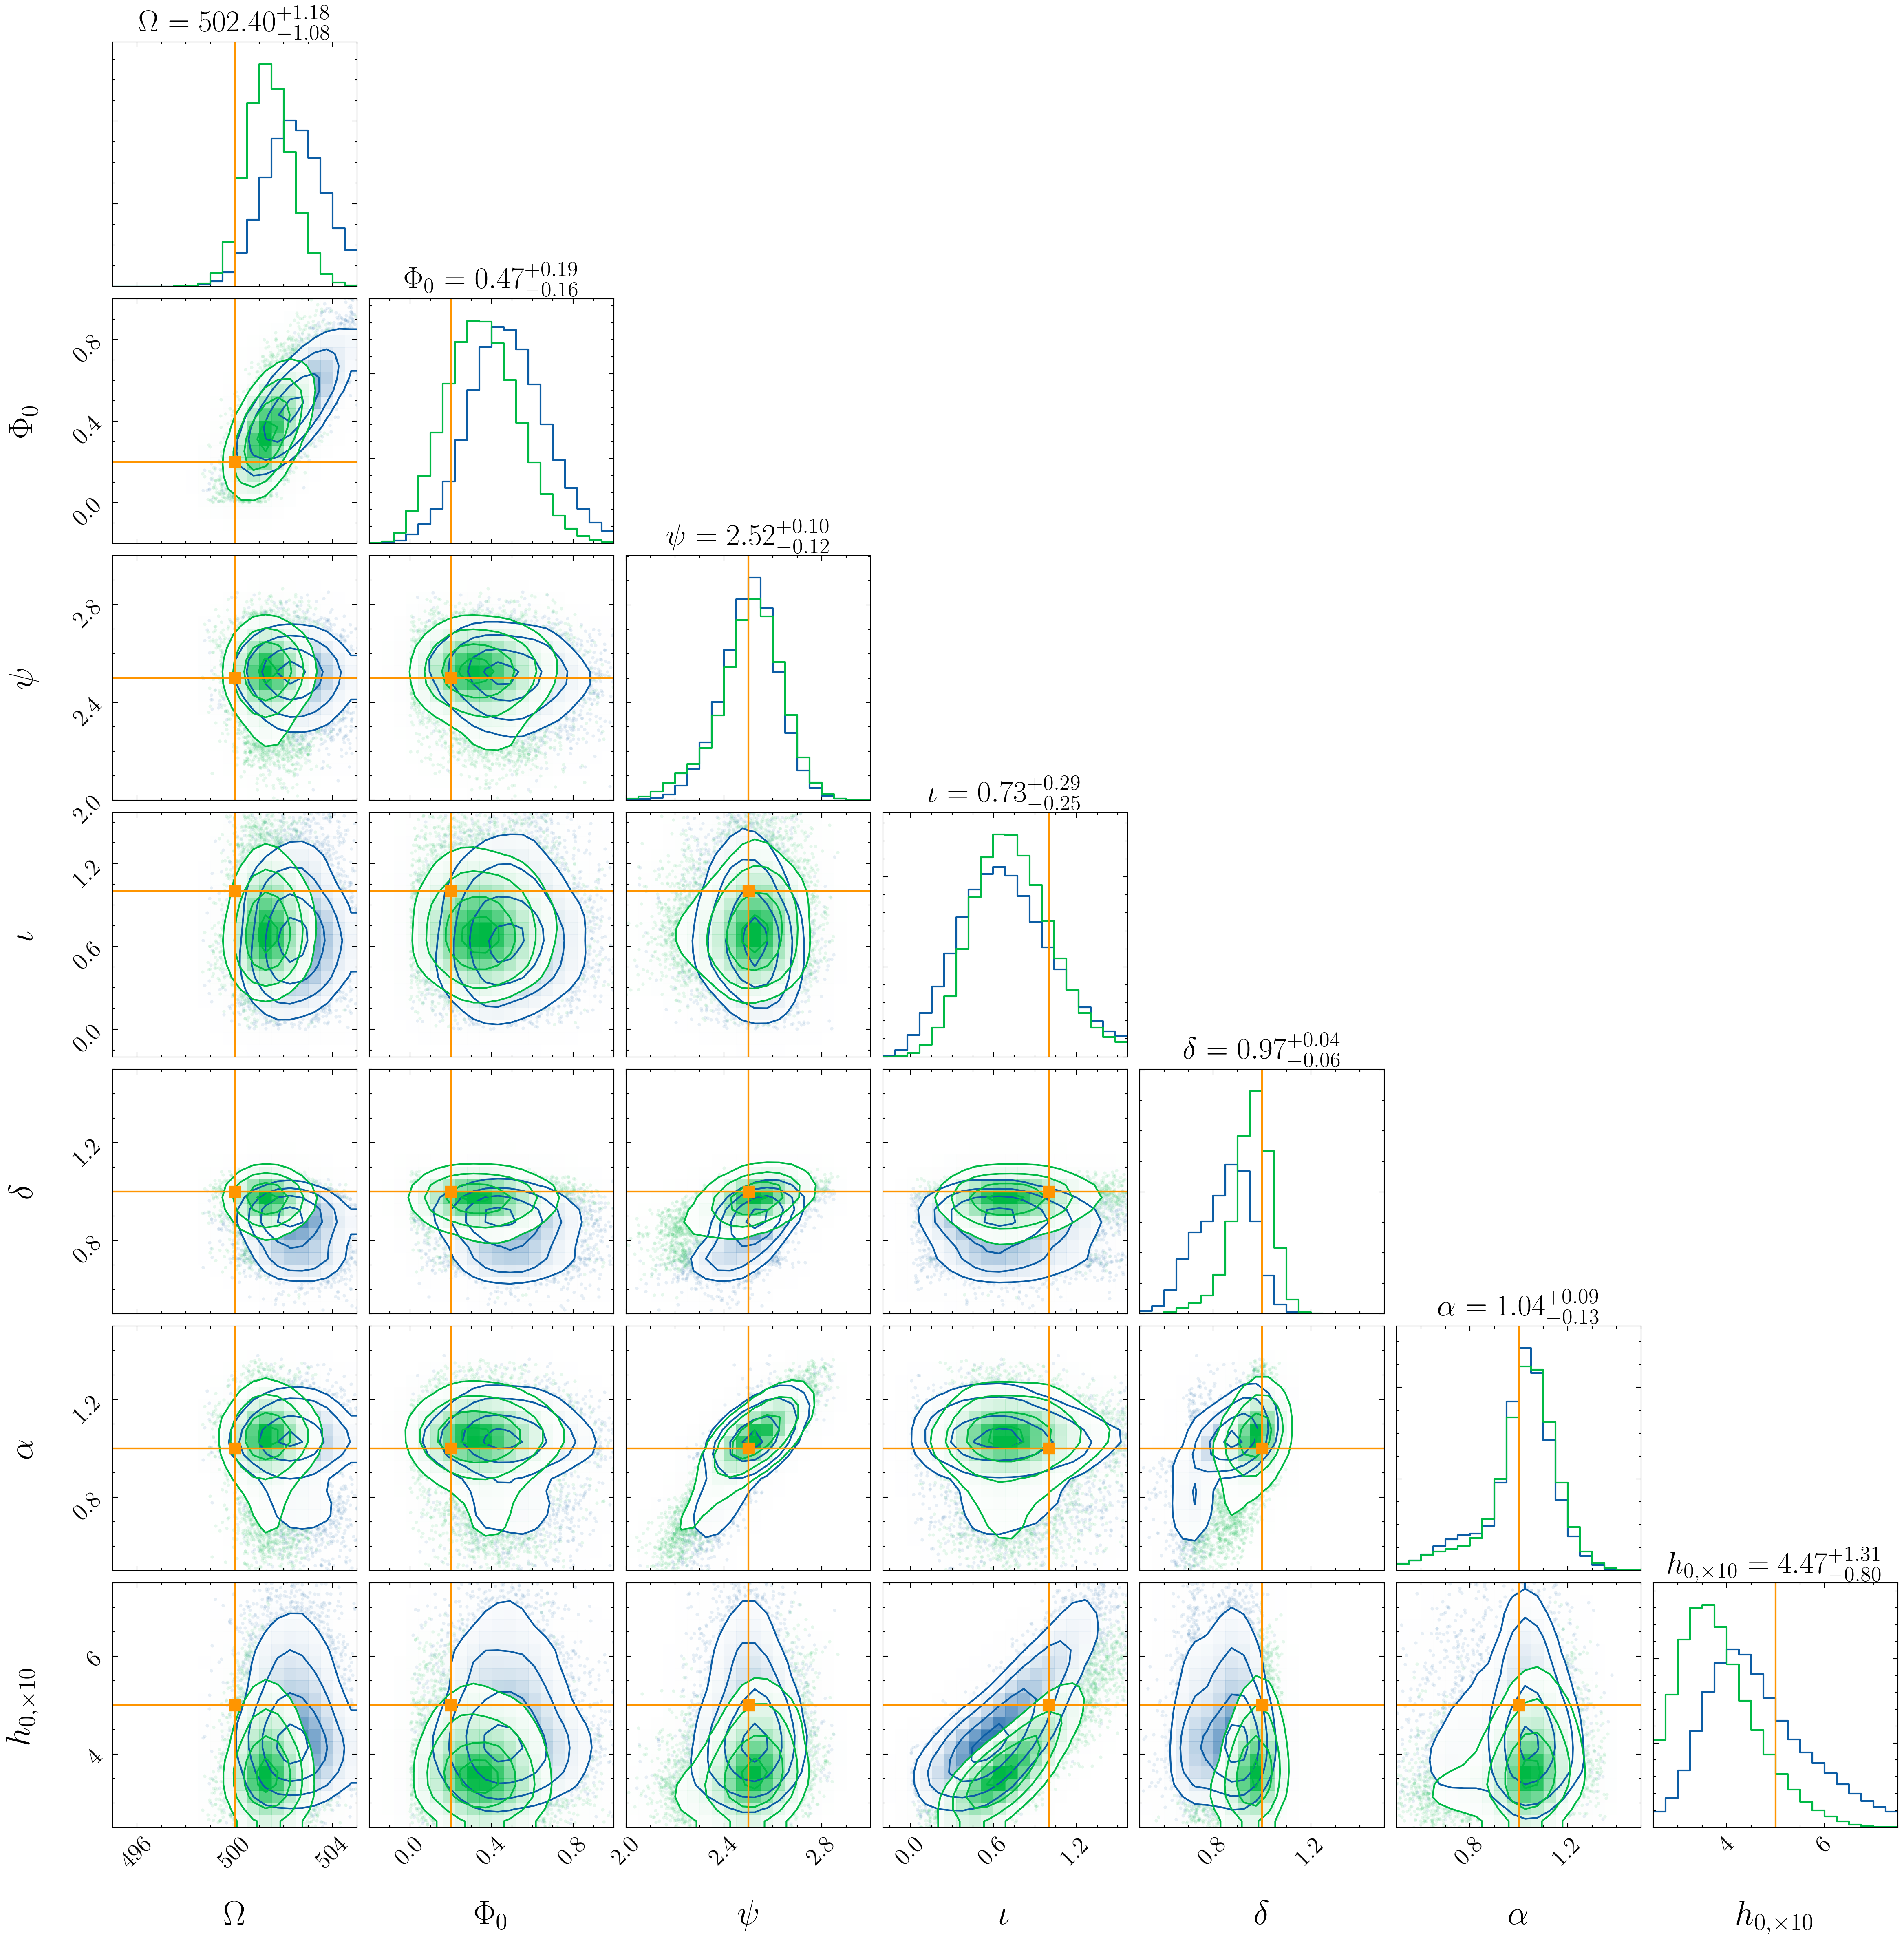
\includegraphics[width=\textwidth, height =\textwidth ]{images/corner_lowSNR}
	\caption{Posterior distribution of the GW source parameters $\boldsymbol{\theta}_{\rm gw}$ for the representative system in Table \ref{tab:parameters_and_priors}, for nine realisations of the noise processes, with curves coloured uniquely. The horizontal and vertical orange lines indicate the true injected values. The contours in the two-dimensional histograms mark the (0.5, 1, 1.5, 2)-$\sigma$ levels after marginalizing over all but two parameters. The one-dimensional histograms correspond to the joint posterior distribution marginalized over all but one parameter. The supertitles of the one-dimensional histograms record the posterior median and the 0.16 and 0.84 quantiles of the median realisation. We plot the scaled variables $10^9 \Omega$ (units: ${\rm rad \, s^{-1}}$) and $10^{15} h_0$. The Kalman filter and nested sampler estimate accurately all seven parameters in ${\boldsymbol{\theta}}_{\rm gw}$. The horizontal axes span a subset of the prior domain for all seven parameters. The known, injected value lies within the 90\% credible interval for 45 out of the 63 combinations of seven parameters and nine noise realizations. There is an appreciable dispersion among the peaks of the one-dimensional posteriors; the maximum coefficient of variation is $43 \%$ for $\Phi_0$, the minimum is $0.02 \%$ for $\Omega$.}
	\label{fig:corner_plot_1}
\end{figure*}

%images/corner_lowSNR_chiF
	\begin{figure}
	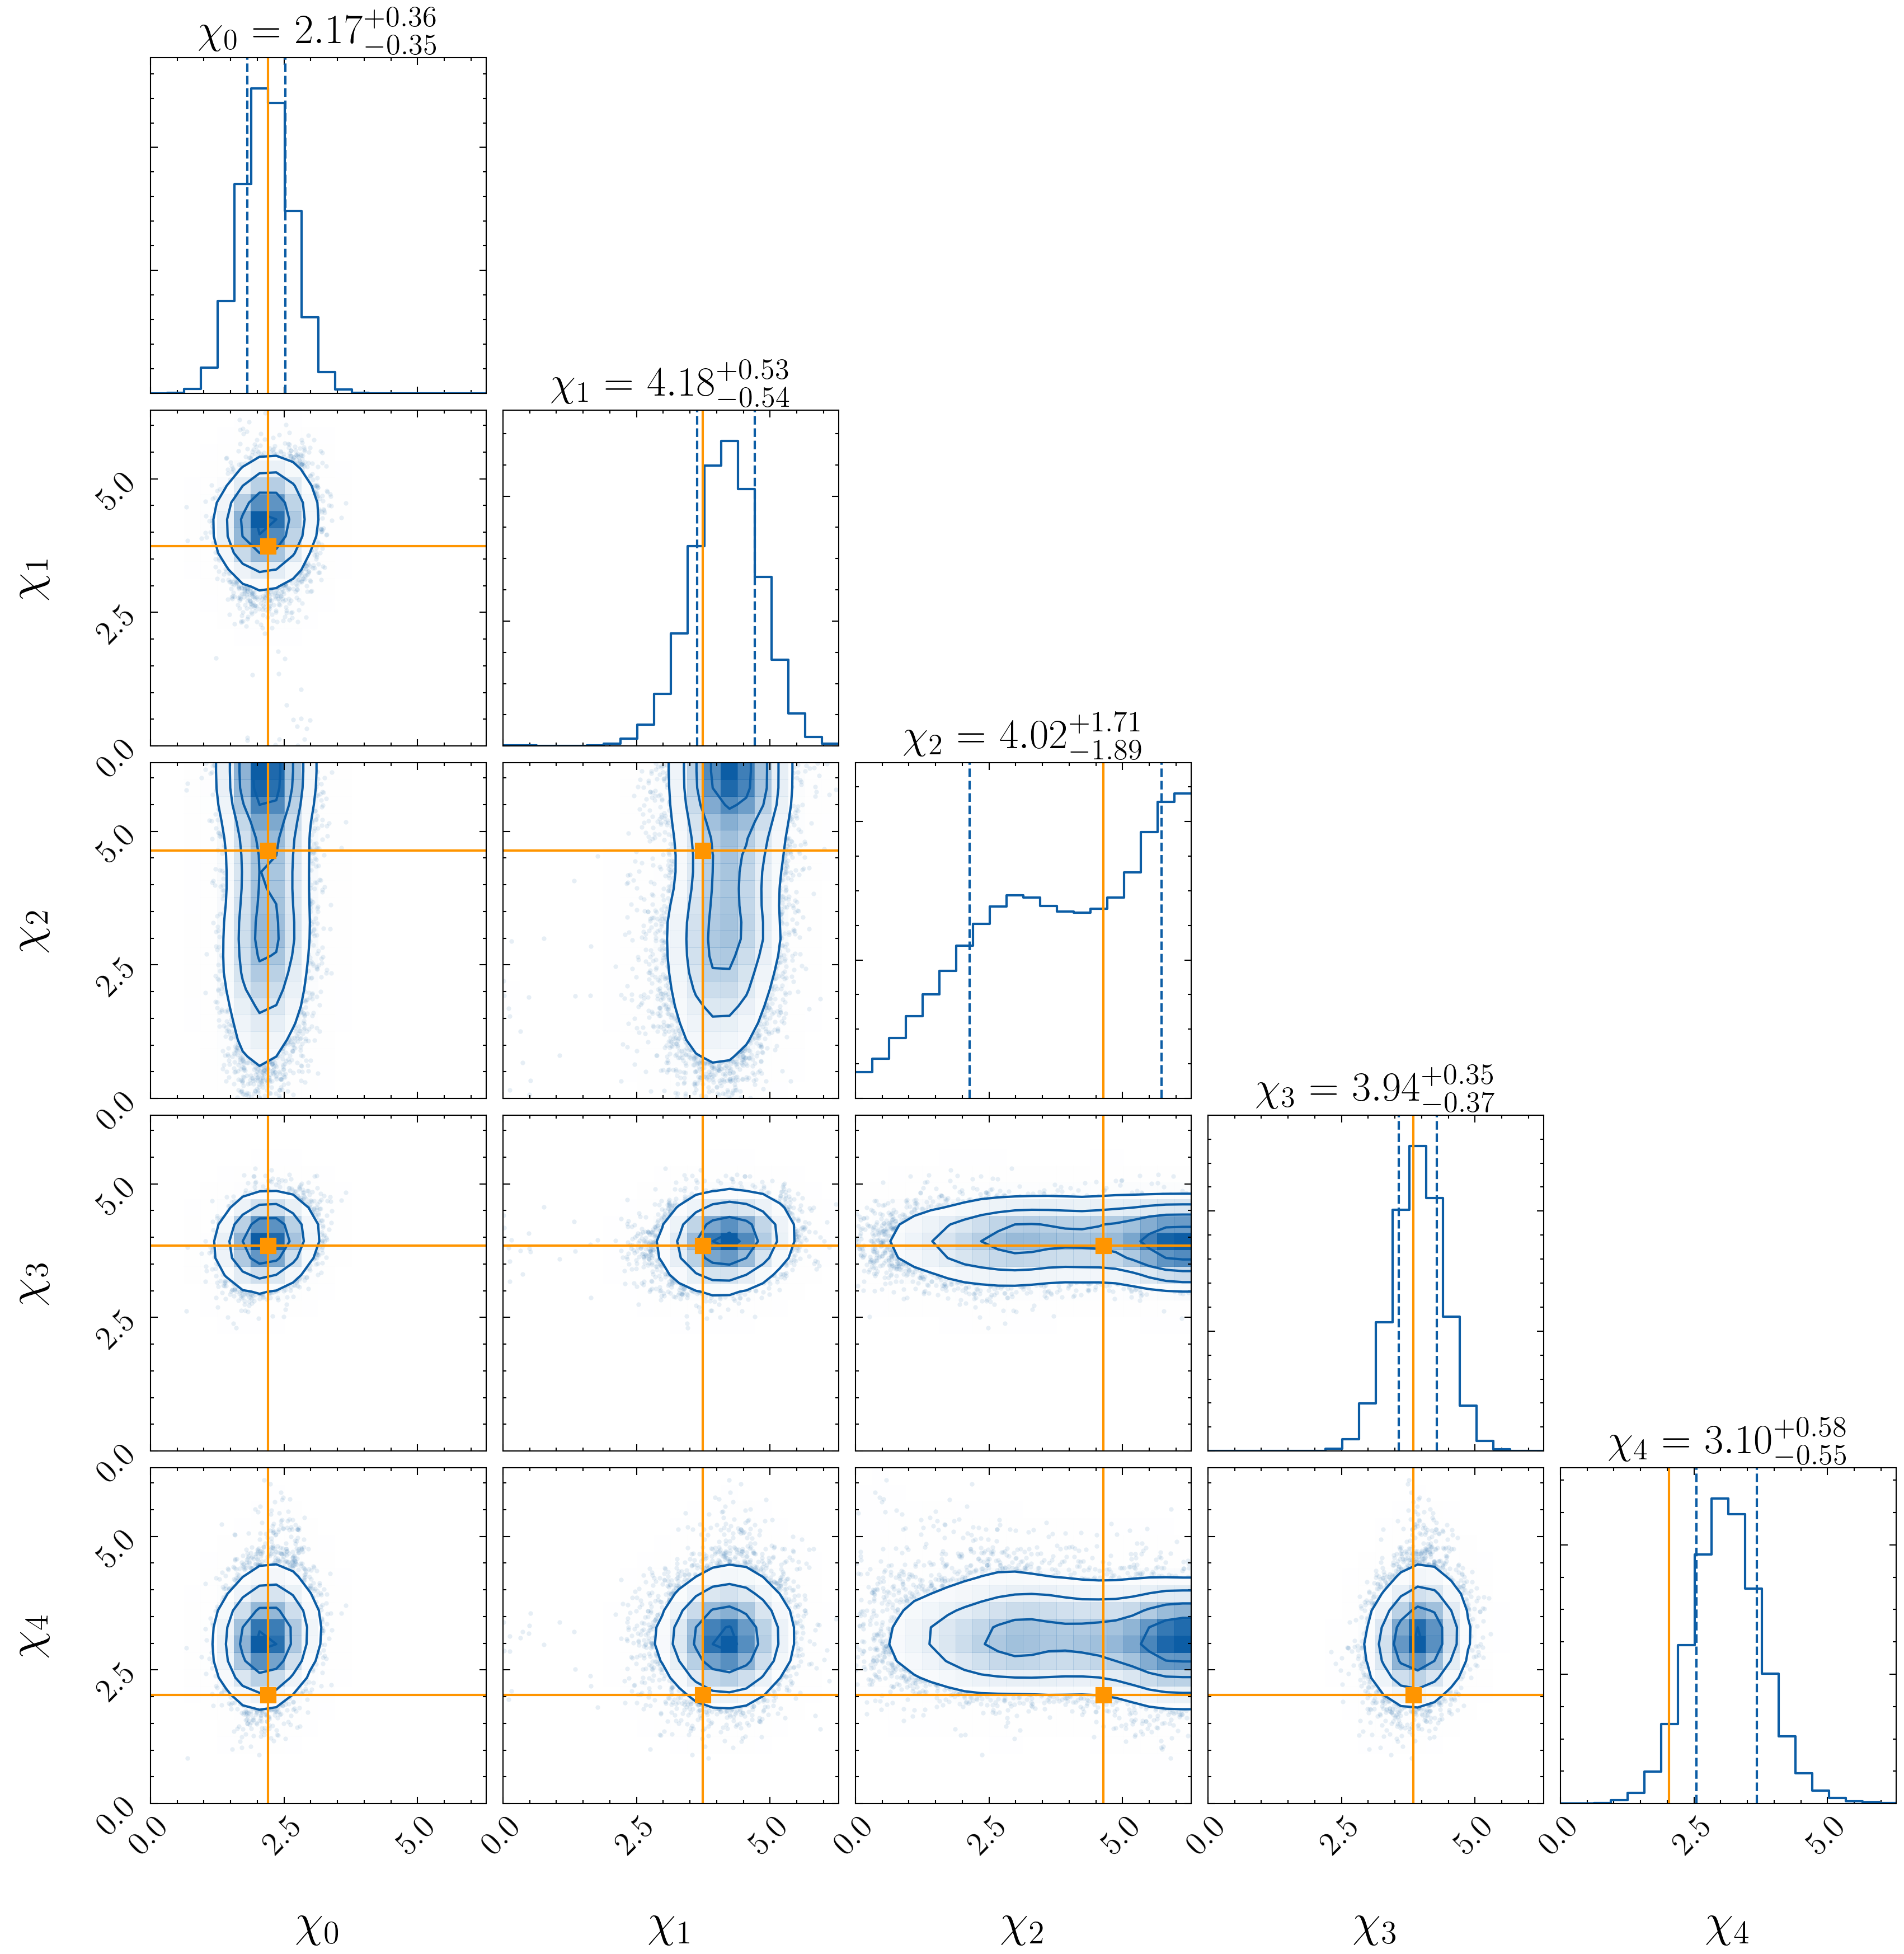
\includegraphics[width=\columnwidth, height =\columnwidth ]{images/corner_lowSNR_chi}
	\caption{Same as Figure \ref{fig:corner_plot_1}	but for five static parameters of $\chi^{(n)}$. Consistent unimodal posteriors are obtained across the nine noise realisations for four out of the five displayed parameters. No consistent posteriors are obtained for $\chi^{(2)}$ (third row, third column), because this pulsar has a similar sky position to that of the synthetic GW source. The known, injected value lies within the 90\% credible interval for 37 out of the 45 combinations of five parameters and nine noise realizations (i.e. $82 \%$). }
	\label{fig:corner_plot_3}
\end{figure}



\subsection{Extension to broader parameter space} \label{sec:parameter_space}
%images/pp_plot_new1
\begin{figure}
	\centering
	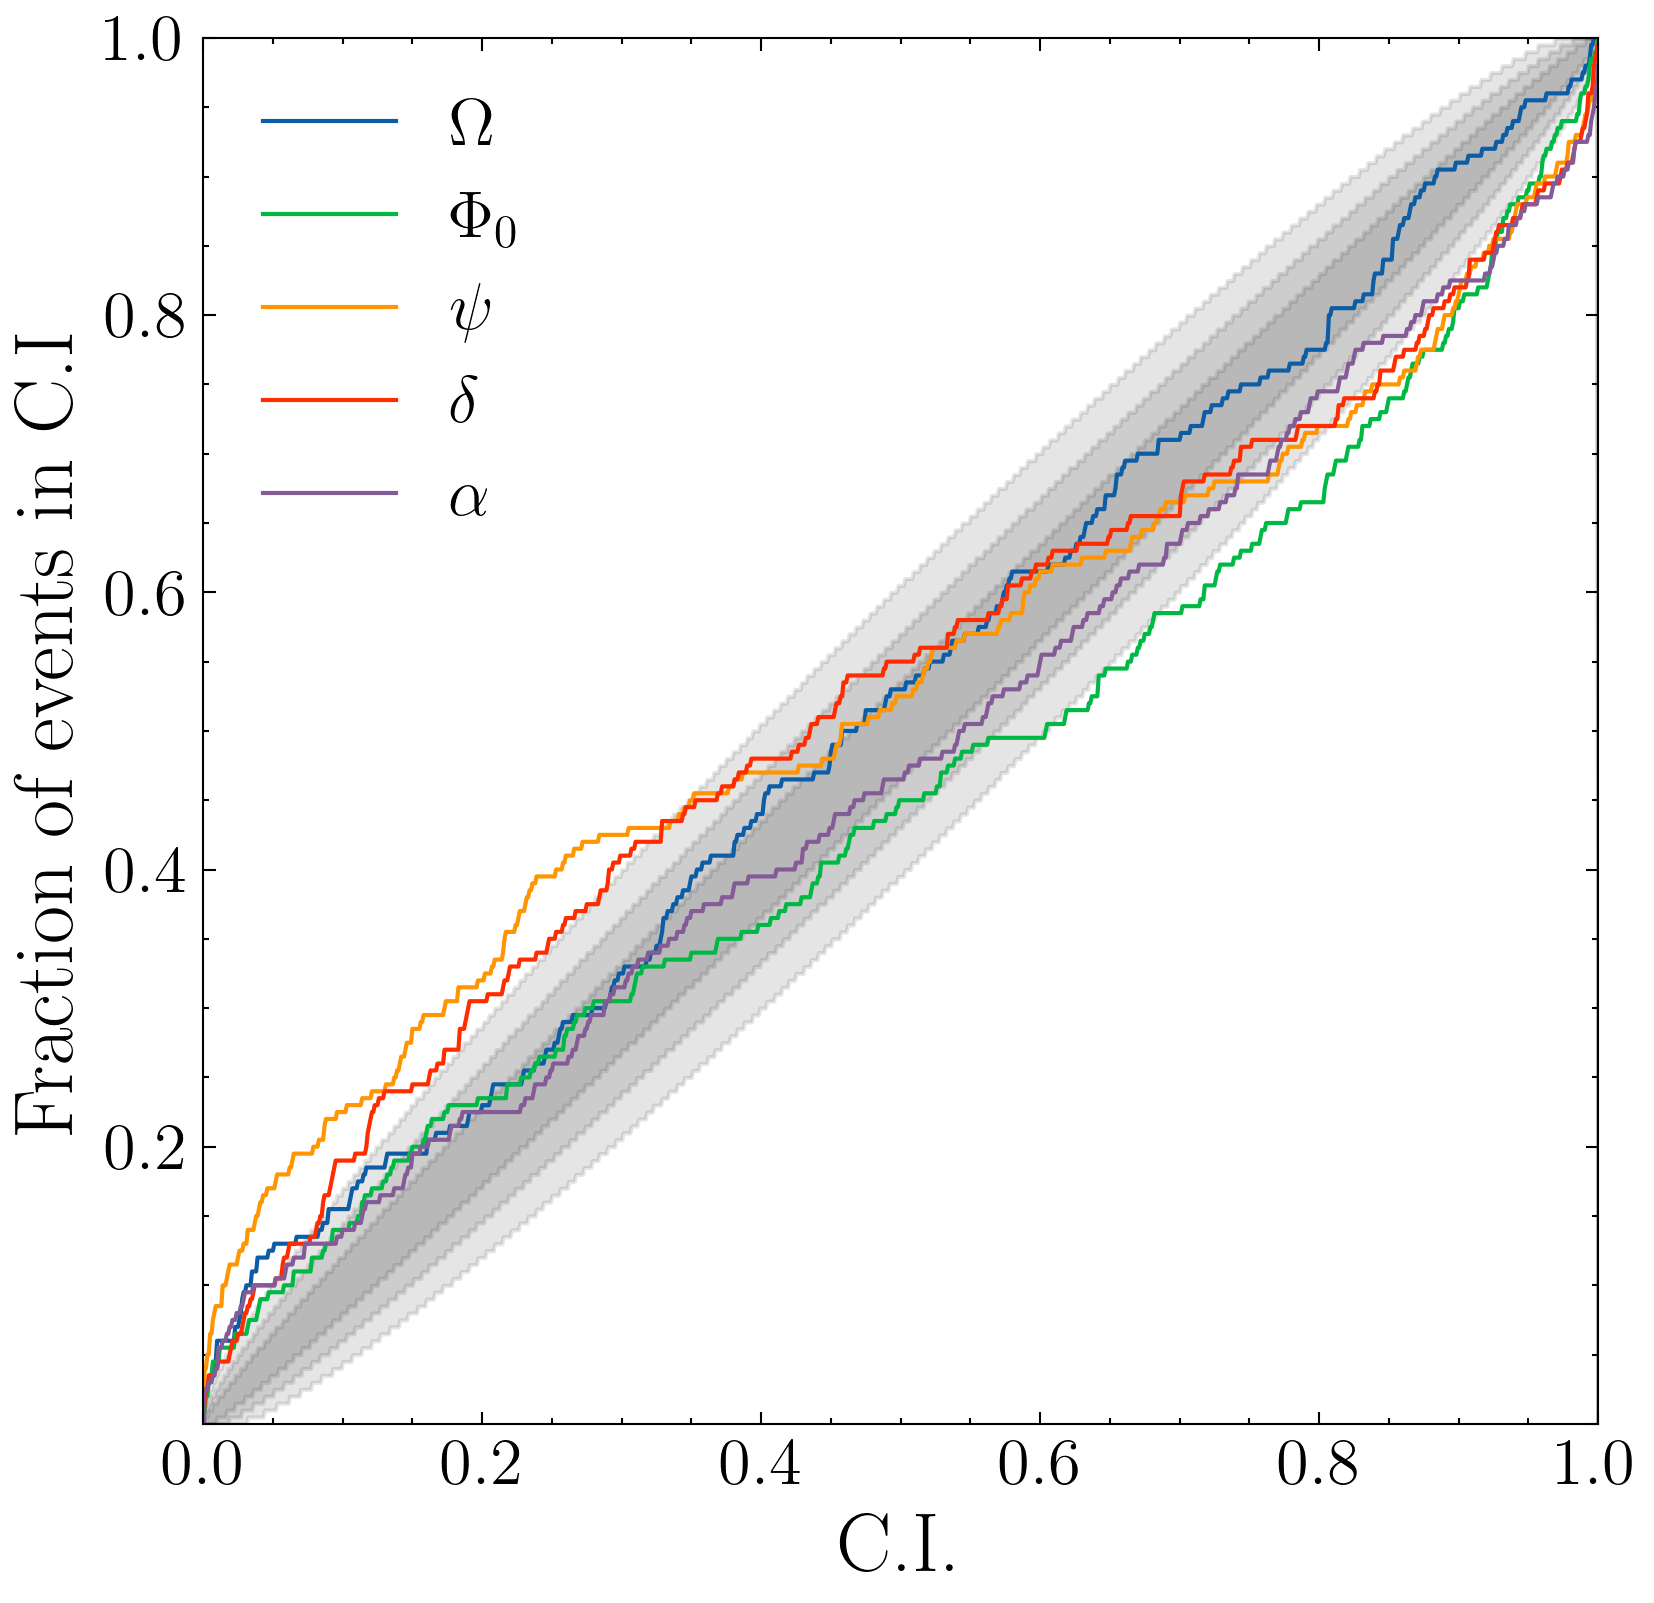
\includegraphics[width=\columnwidth]{images/pp_plot_canonical500}
	\caption{Fraction of injections included within a given credible interval of the estimated posterior, as a function of the credible interval itself (i.e. PP plot). The injections are 200 simulated GW sources generated by drawing randomly five parameters in $\boldsymbol{\theta}_{\rm gw}$ from the prior distributions in Table \ref{tab:parameters_and_priors}. Each coloured curve corresponds to a different parameter (see legend). The parameters $h_0$ and $\iota$ are fixed at $5 \times 10^{-15}$ and 1.0 rad respectively in order to maintain an approximately constant SNR. The grey shaded contours label the $1\sigma$, $2\sigma$ and 3$\sigma$ confidence intervals. For parameters with well estimated posteriors, the PP curve should fall along the diagonal of unit slope. $\Omega$ and $\alpha$ are generally well-estimated (i.e. the curves lie close to the unit diagonal). The remaining three parameters, $\psi$, $\phi_0$ and $\delta$ show modest evidence of being over-constrained and stray outside the shaded region.}
	\label{fig:parameter_space}
\end{figure}
Section \ref{sec:pe_and_ms} focuses on a single representative system, summarised in Table \ref{tab:parameters_and_priors}. In this section we test the method for various systems, varying the SMBHB source parameters $\boldsymbol{\theta}_{\rm gw}$ through astrophysically relevant ranges. The aim of this section is to confirm that the analysis scheme can be applied across an astrophysically relevant parameter space and that the arbitrary choice of $\boldsymbol{\theta}_{\rm gw}$ in Section \ref{sec:pe_and_ms} is not particularly advantageous by accident. \newline 


We analyse 200 injections constructed by fixing $h_0 = 5 \times 10^{-15}$, $\iota =1.0$ rad and drawing the remaining five elements of $\boldsymbol{\theta}_{\rm gw}$ randomly from the prior distributions defined in Table \ref{tab:parameters_and_priors}. We fix $h_0$ and $\iota$ in order to maintain an approximately constant signal-to-noise ratio (SNR) across the 200 injections. For each injection we compute the posterior distribution of ${\boldsymbol{\theta}}_{\rm gw}$. The static pulsar parameters $\boldsymbol{\theta'}_{\rm psr}$ are as specified in Section \ref{sec:synthetic_data} and Table  \ref{tab:parameters_and_priors}. \newline 


It is prohibitive to produce corner plots analogous to Figure \ref{fig:corner_plot_1} for 200 injections and seven elements of $\boldsymbol{\theta}_{\rm gw}$. Therefore, in order to summarise the results we use a parameter-parameter (PP) plot \citep{doi:10.1198/106186006X136976}. A PP plot displays the fraction of injections included within a given credible interval of the estimated posterior, as a function of the credible interval itself. In the ideal case of perfect recovery, the PP plot should be a diagonal line of unit slope. The results are displayed in Figure \ref{fig:parameter_space}.  
The shaded grey contours enclose the $1\sigma$, $2\sigma$, and $3\sigma$ significance levels for 200 injections. The curves for the five parameters generally exhibit the discussed linear behaviour. Some parameters are consistently well estimated across the parameter space; the blue curve for $\Omega$ is consistently contained within the 2-$\sigma$ shaded region. 


Conversely some parameters e.g. $\psi$ stray outside the $1\sigma$ bounded region and show evidence of being over constrained; there are more injections contained within lower-value credible intervals than would be expected statistically, and less injections contained within higher-value credible intervals. 

With a strain of X, we are close to the nosie floor (see e.g. figure X), so small variations in 



Inspecting the individual resulting corner plots for each of the 200 injections, it is evident that for a minority of SMBHB sources the method either does not converge to a consistent unimodal one-dimensional posterior, or else a posterior is calculated but is slightly offset, not symmetric about the injected value. 


due to challenge of etimateng phi


The 

At this signal-to-noise ratio 


the polarisation angle does stray above /below 


At low SNR the ability to resolve the depends upon the noise realisation and the source location. The antenna pattern function formed by the NANOGrav 12.5 year pulsars is sensitive to different parts of the sky. Areas with lower sensitivity may need to be  



Conversely the ability to infer $\Omega$ depends less on sky position or values. 



\section{Earth terms vs pulsar terms}\label{sec:earth_vs_psr}
In Section \ref{sec:rep_example1} we have validated the state-space analysis scheme when the pulsar terms are included in the inference model. In this section, critically, we compare the effect of including the pulsar-term in the model (i.e. using Equation \eqref{eq:g_func_trig_chi}), as opposed to the omitting the pulsar-term (i.e. Equation \eqref{eq:g_func_trig_earth}). We do this using the specific representative case of the individual quasi-monochromatic SMBHB source described in Table \ref{tab:parameters_and_priors}. We refer to the model where the pulsar-term is included alongside the Earth term as $\mathcal{M}_{\rm P \& E}$. We refer to the model where the pulsar-term is omitted as 
$\mathcal{M}_{\rm E}$. Model $\mathcal{M}_{\rm P \& E}$ is parameterised by $\boldsymbol{\theta}'$. Model $\mathcal{M}_{\rm E}$ is parameterised by $\boldsymbol{\theta}_{\rm E} = \boldsymbol{\theta}_{\rm gw} \cup \boldsymbol{\theta}'_{\rm psr}$. Both models are applied to identical realisations of the data, generated using the procedure as described in Section  \ref{sec:synthetic_data}. The priors on the static parameters in each model are also identical, with the addition of a uniform prior on $\chi^{(n)}$ for $\mathcal{M}_{\rm P \& E}$, as described in Appendix \ref{sec:set_priors}. \newline 


In Section \ref{sec:psr_v_earth_pe} we compare the accuracy of the estimates of $\boldsymbol{\theta'}$, $\boldsymbol{\theta}_{\rm E}$ returned by the respective models. In Section \ref{sec:psr_v_earth_bayes} we compare the minimal detectable strain for the two models. 




\subsection{Accuracy of parameter estimation}\label{sec:psr_v_earth_pe}

In this section apply we apply the Kalman filter in conjunction with nested sampling in order to infer the joint posterior distribution for the static parameters of each model. For $\mathcal{M}_{\rm E}$ we apply the Kalman filter using Equation \eqref{eq:g_func_trig_earth} to return $\mathcal{L}(\boldsymbol{Y}| \boldsymbol{\theta}_{\rm E})$. The likelihood returned by the Kalman filter is then used by nested sampling in order to estimate $p(\boldsymbol{\theta}_{\rm E} | \boldsymbol{Y})$. For $\mathcal{M}_{\rm P \& E}$ we apply the Kalman filter using Equation \eqref{eq:g_func_trig_chi} to return $\mathcal{L}(\boldsymbol{Y}| \boldsymbol{\theta}')$. The likelihood returned by the Kalman filter is then used by nested sampling in order to estimate $p(\boldsymbol{\theta'} | \boldsymbol{Y})$. The settings of the nested sampler (for example the number of live points, see Appendix \ref{sec:nested_sampling}) are identical for both models. \newline 

We consider two representative systems. The first is a ``low-SNR" system with $h_0 = 5 \times 10^{-15}$, i.e. the exact system described in Table \ref{tab:parameters_and_priors}. The second is a ``high-SNR" system which has the same static injection parameters, but with an increased $h_0 = 10^{-12}$. The ``high-SNR" system is considered in order to evaluate the parameter estimation accuracy, and in particular any potential bias, without confusion from the measurement noise. In order to enable a clear comparison between the posterior probability distributions calculated using the two models, in this section we consider a single noise realisation of the synthetic data $\boldsymbol{Y}$. The results quoted are consistent across different noise realisations. \newline 


The results for the seven parameters of  $\boldsymbol{\theta}_{\rm gw}$ are shown in Figure \ref{fig:corner_plot_compare_high} for the high-SNR system and in Figure \ref{fig:corner_plot_compare_low} for the low-SNR system. The corner plot is arranged identically to Figure \ref{fig:corner_plot_1}, however the different coloured curved now correspond to different inference models, rather than different realisations of $\boldsymbol{Y}$. The blue curves are the results derived using $\mathcal{M}_{\rm E}$. The green curves are the results derived using $\mathcal{M}_{\rm P \& E}$. \newline 
		
For the high-SNR case, Figure \ref{fig:corner_plot_compare_high}, the one-dimensional posteriors for the Earth-term model are evidently biased, as was observed in K24, as well as \cite{Zhupulsarterms} and \cite{Chen2022}. Particular biases are observed in $\psi, \iota $ and $\alpha$, with the blue posterior displaced with respect to the orange injection line. For example, for $\iota$, whilst the injected value is contained within the 90\% credible interval, the median of the posterior of the Earth-term model is shifted from the injected value by 0.35 radians. The inclusion of the pulsar terms corrects for this bias; the green one-dimensional exhibit no bias and are generally symmetric about the injected value. Moreover, for every pair of parameters the injection values are contained within the 2-sigma equivalent contours for the pulsar-term model, which is not true in the Earth-terms case. \newline 


We define a root-mean-square relative error to quantify the accuracy of the one-dimensional posteriors with respect to the injection value as
\begin{equation}
\Delta_{\rm M}(\theta) = \sqrt{\frac{1}{K}\sum_{k=1}^{K} \frac{ \left[p_k(\theta) - \hat{\theta}\right]^2}{\hat{\theta}}} \ , \label{eq:mean_rel_error}
\end{equation}
where $p_k(\theta)$ is the $k$-th one-dimensional posterior sample for parameter $\theta$, $K$ is the total number of samples, $\hat{\theta}$ is the true injection value, and the subscript $M \in \{ \text{earth, pulsar} \}$ indicates whether the posterior is estimated using Equation \eqref{eq:g_func_trig_earth} or Equation \eqref{eq:g_func_trig} respectively. The dependence of $p_k(\theta)$ on $M$ is implied. The values of $\Delta_{\rm M}(\theta)$ for each parameter in Figure \ref{fig:corner_plot_compare_high} are summarised in Table \ref{tab:posterior_errors}. The difference in the error between the two models, $\Delta_{\rm earth}(\theta)-\Delta_{\rm pulsar}(\theta)$ is also presented. For every parameter $\Omega$, $\Delta_{\rm earth}(\theta)-\Delta_{\rm pulsar}(\theta)$ is positive, indicating that the parameter estimates are more accurate using the pulsar terms. In some cases the difference is modest;  $\Omega$ is recovered with high accuracy by both models such that $\Omega$, $\Delta_{\rm earth}(\Omega)-\Delta_{\rm pulsar}(\Omega) = 6.7 \times 10^{-3}$ rad. The improvement from using the pulsar terms is largest for $\iota$, with $\Delta_{\rm earth}(\iota) - \Delta_{\rm pulsar}(\iota)  = 0.24$ rad. As a percentage change, i.e. $1 - \Delta_{\rm earth}(\theta)/\Delta_{\rm pulsar}(\theta)$, the improvement from using $\mathcal{M}_{\rm P \& E}$ over $\mathcal{M}_{E}$ ranges from 61\% for $\Omega$ to 99\% for $\psi$ and $\alpha$. These improvements are consistent across noise realisations. \newline 


For the low-SNR case,  Figure \ref{fig:corner_plot_compare_low}, there is less of a notable improvement in the parameter estimates. Qualitatively, the green and blue one-dimensional posteriors are generally overlaid. The two-dimensional contours suggest a slight improvement through using the pulsar terms, but the difference is modest. The root-mean-square relative error $\Delta_{\rm M}(\theta)$ for the low SNR case is also reported in Table \ref{tab:posterior_errors}. We see that the error is larger for every element in $\boldsymbol{\theta}_{\rm gw}$ than in the high SNR case, as expected. The inclusion of the pulsar terms improve the estimates for five out of the seven static parameters; $\Delta_{\rm earth}(\theta)-\Delta_{\rm pulsar}(\theta)$ is positive for all parameters except $\psi$ and $h_0$. However it is hard to draw strong conclusions; for different realisations of the noise different parameters exhibit either improvement or deterioration in $\Delta_{\rm M}(\theta)$. We conclude that the inclusion of the pulsar terms does not significantly improve the parameter estimates in the low-SNR case. This is intuitive since the system is highly noise dominated such that an increasing model complexity does not aid parameter estimates. Whilst the inclusion of the pulsar terms only modestly improve the accuracy of the parameter estimates in the case of low-SNR, we will show in Section \ref{sec:psr_v_earth_bayes} that they are important for increasing the detection probability for a given signal strength. \newline 
		
	\begin{figure*}
	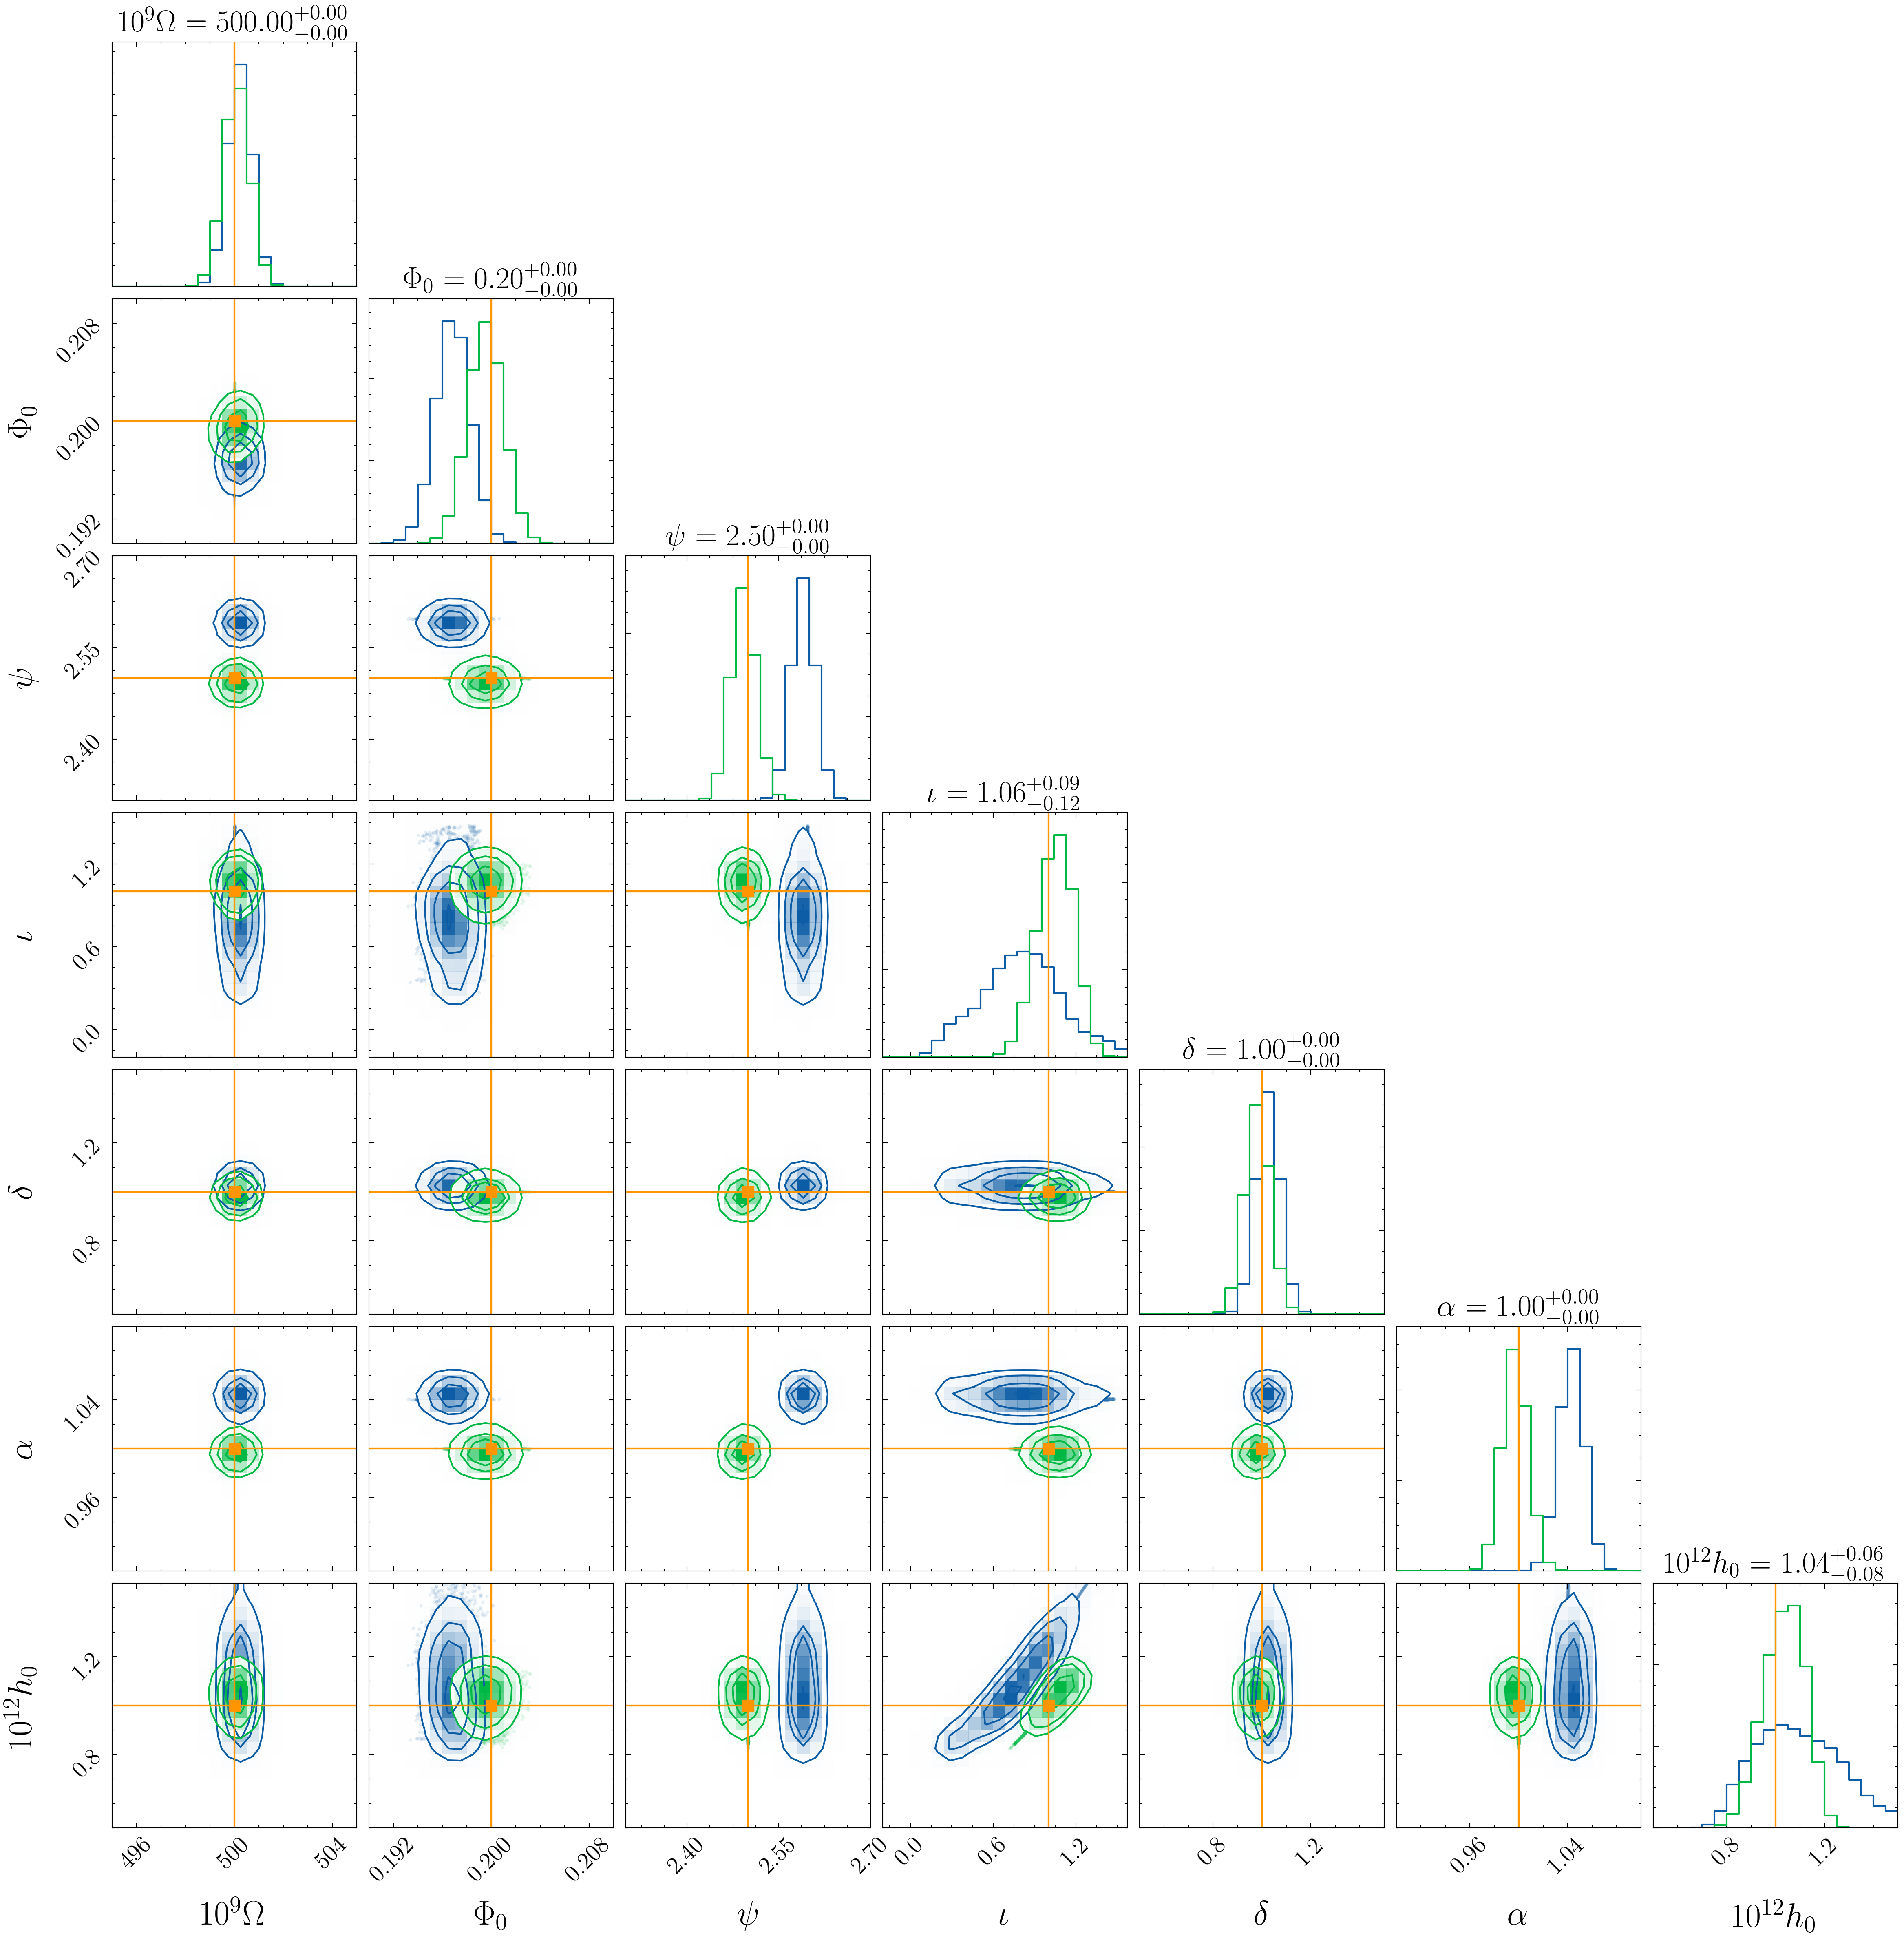
\includegraphics[width=\textwidth, height =\textwidth ]{images/corner_highSNR_compare}
	\caption{Posterior distribution of the GW source parameters $\boldsymbol{\theta}_{\rm gw}$ for the representative system described in Table \ref{tab:parameters_and_priors}, with $h_0 = 10^{-12}$, for a single realisation of the system noise. The blue curves are the posteriors derived using the Earth-term model, Equation \eqref{eq:g_func_trig_earth}, the green curves using the pulsar-term model, Equation \eqref{eq:g_func_trig}. The vertical orange lines indicate the true injected values. The contours in the 2D histograms denote the (0.5, 1, 1.5, 2)-$\sigma$ levels. The supertitles of the one-dimensional histograms record the posterior medians and the 0.16 and 0.84 quantiles of the green curves, i.e. the pulsar-term model. We plot the scaled variables $10^9 \Omega$ (units: rad s$^{-1}$) and $10^{12} h_0$. Some parameters (e.g. $\psi, \iota$) exhibit a bias when using the Earth-term model which is absent when using the pulsar-term model.}
	\label{fig:corner_plot_compare_high}
\end{figure*}


\begin{figure*}
	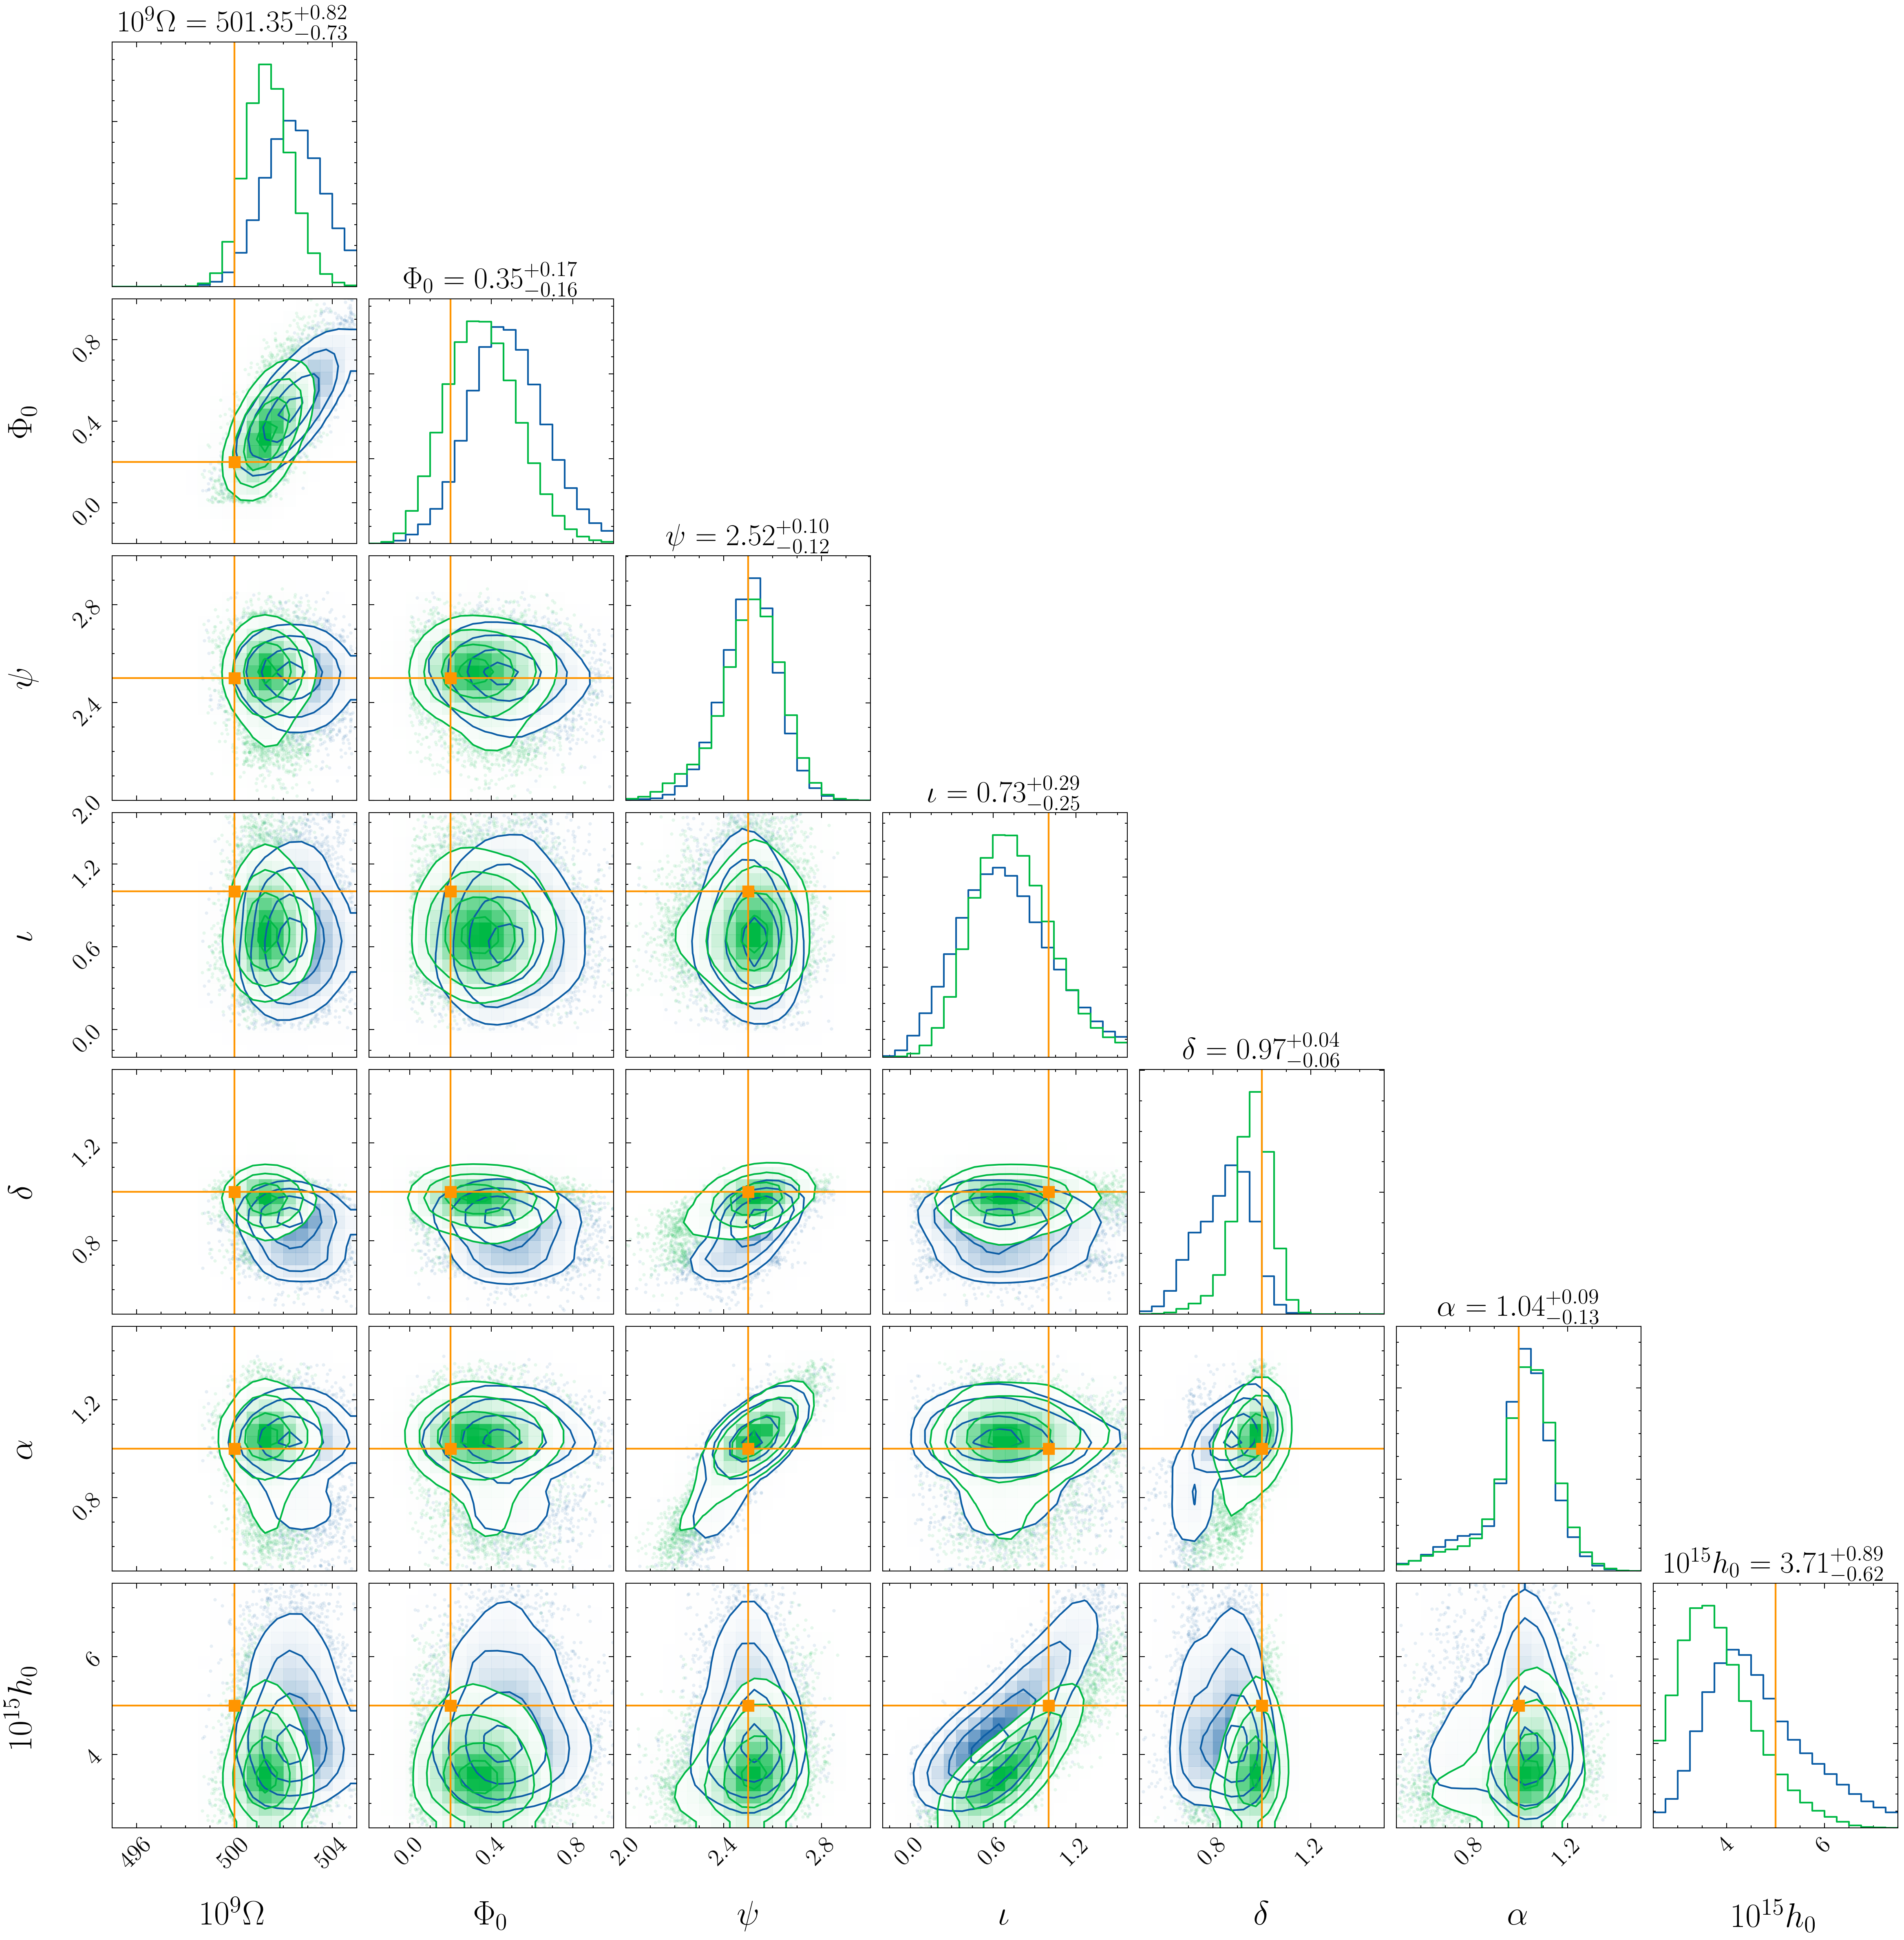
\includegraphics[width=\textwidth, height =\textwidth ]{images/corner_lowSNR_compare}
	\caption{Same as Figure \ref{fig:corner_plot_compare_high}, but for a low-SNR system with $h_0 = 5 \times 10^{-15}$. The posterior distributions from the Earth-term and pulsar-term models are generally overlaid }
	\label{fig:corner_plot_compare_low}
\end{figure*}



\begin{table}
	\centering
	%	\resizebox{\textwidth}{!}{%
		%	\renewcommand{\arraystretch}{1.0} % Default value: 1
		\begin{tabular}{lcllc}
			\toprule
			&$\theta$ & $\Delta_{\rm earth}(\theta)$ & $\Delta_{\rm pulsar}(\theta)$ & $\Delta_{\rm earth}(\theta) - \Delta_{\rm pulsar}(\theta)$   \\
			\hline
			\multirow{7}{2mm}{High SNR} & $\Omega$       & 0.011& 0.0043& 0.00671\\
			& $\Phi_0$ &0.00332 &0.00115 &0.00217\\
			& $\psi$ &0.0968 &0.000653 &0.0962 \\
			& $\iota$ & 0.343 &0.106 &0.237 \\
			& $\delta$ & 0.00187 &0.000285 &0.00158 \\
			&$\alpha$ &0.0403 &0.000435 &0.0399 \\
			&$h_0$ & 0.227 &0.075 &0.152 \\
			\hline
			\multirow{7}{2mm}{Low SNR} & $\Omega$       & 2.7 &1.6& 1.09 \\
			& $\Phi_0$ &0.335 &0.229 &0.106 \\
			& $\psi$ &0.112 &0.123 &-0.0119 \\
			& $\iota$ & 0.443 &0.37 &0.0724 \\
			& $\delta$ & 0.181 &0.0782 &0.103 \\
			&$\alpha$ &0.145 &0.139 &0.00637 \\
			&$h_0$ & 1.12 &1.41 &-0.291 \\
			\bottomrule
		\end{tabular}
		\caption{Root-mean-square relative error $\Delta_{\rm M}(\theta)$, Equation \eqref{eq:mean_rel_error}, in the one-dimensional posteriors calculated using the Earth-term model (M = earth, Equation \eqref{eq:g_func_trig_earth}) and the pulsar-term model (M=pulsar, Equation \eqref{eq:g_func_trig}) for the elements $\theta \in \boldsymbol{\theta}_{\rm gw}$. The injection values are as summarised in Table \ref{tab:parameters_and_priors}. The top and bottom halves of the table contain the high-SNR ($h_0 = 10^{-12}$) and low-SNR ($h_0 = 5 \times 10^{-15}$) cases respectively.  For all parameters the units are in rad, except for $h_0$ which is dimensionless. The rightmost column quotes the difference in the mean relative error between the models for each parameter; a negative value indicates that the pulsar-term model is more accurate.}
		\label{tab:posterior_errors}
	\end{table}



\subsection{Detectability vs $h_0$}\label{sec:psr_v_earth_bayes}
		
		\begin{figure}
			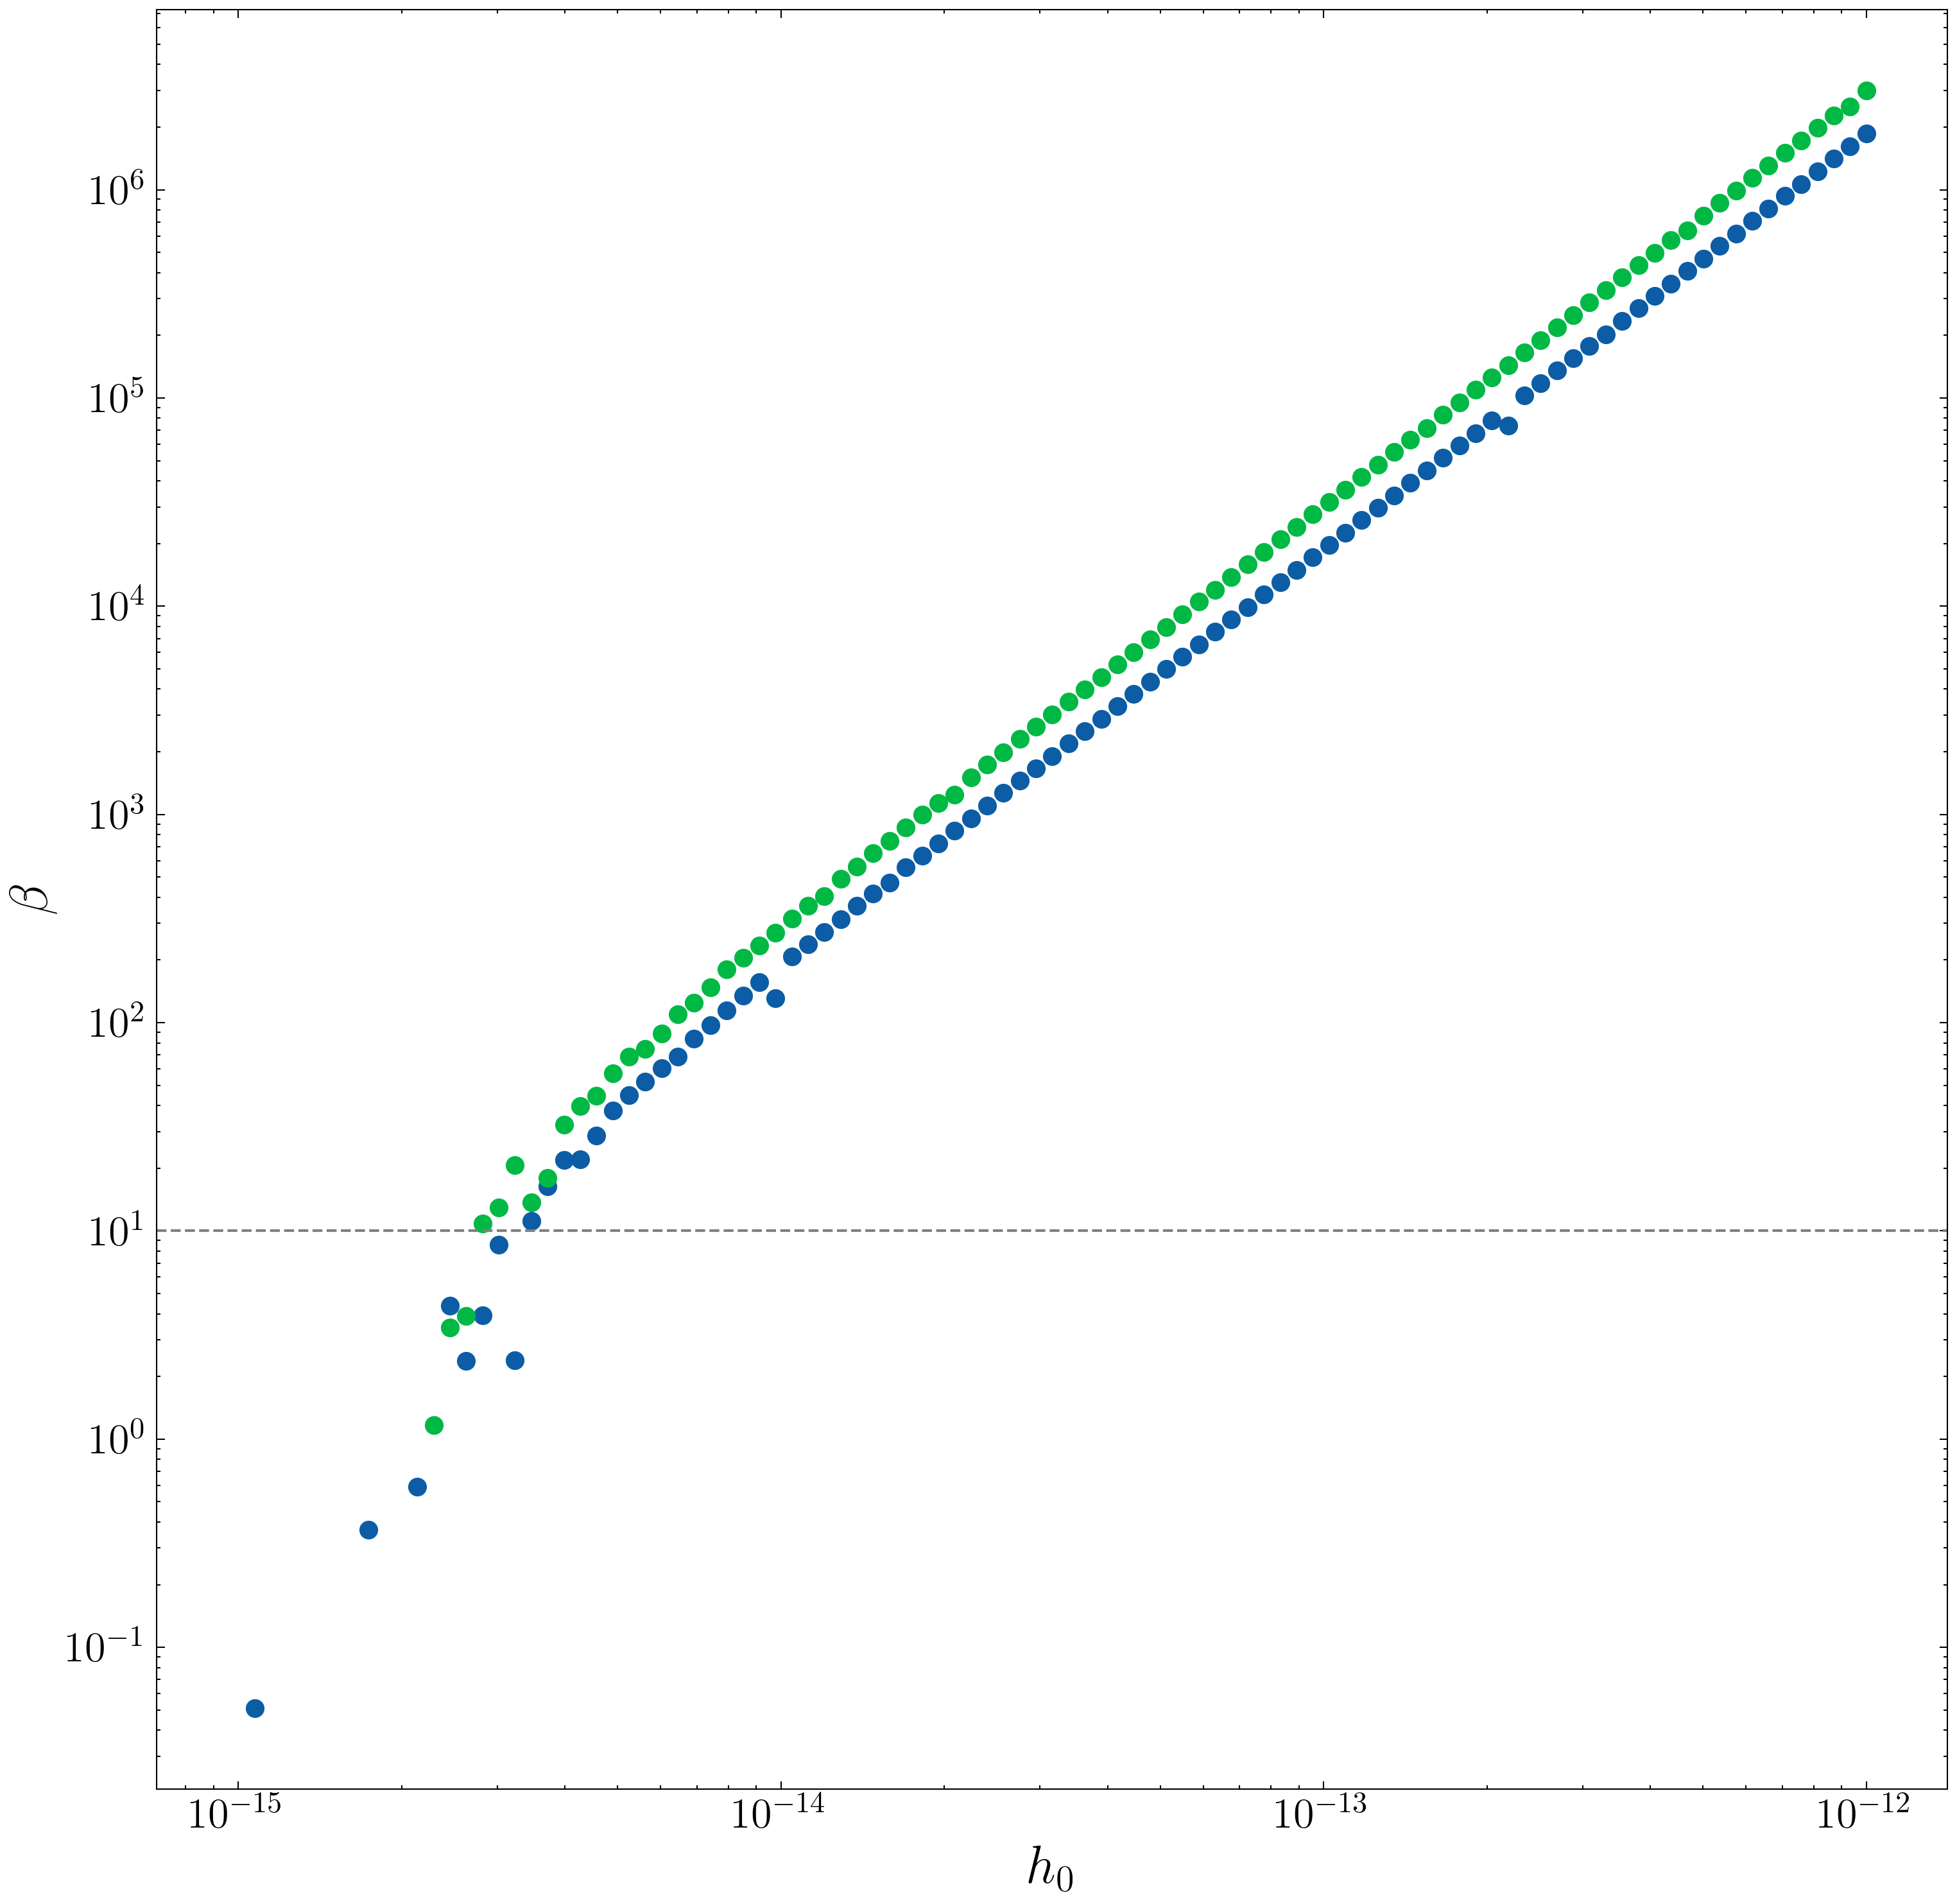
\includegraphics[width=\columnwidth, height = \columnwidth ]{images/CanonicalBayesPlot2000} 	
			\caption{Bayes factor (odds ratio) $\beta$ between the competing models $\mathcal{M}_1$ (GW present in data) and $\mathcal{M}_0$ (GW not present in data) at different GW strains, $h_0$, for the representative example in Table \ref{tab:parameters_and_priors}. The horizontal grey dashed line labels an arbitrary detection threshold, $\beta = 10$. The minimum detectable strain, for $\beta < 10$, equals $4 \times 10^{-15}$. Missing points for $\beta \lesssim 10$ occur when noise subverts the hierarchical relationship between $\mathcal{M}_0$ and $\mathcal{M}_1$ (see Section \ref{sec:detection}).}
			\label{fig:bayes1}
		\end{figure}
The evidence integral $\mathcal{Z}$ returned by nested sampling, Equation \eqref{eq:model_evidence}, is the probability of the data $\boldsymbol{Y}$ given a model $\mathcal{M}_i$. We define $\mathcal{M}_{\rm null}$ as the null model that assumes no GW exists in the data. This is equivalent to setting $g^{(n)}(t)=1$ in Equation \eqref{eq:g_func_trig}. The support in the data for the presence of a GW signal, described by model $\mathcal{M}_i$, over the absence of a GW signal is quantified via a Bayes factor
		\begin{equation}
			\beta_i = \frac{\mathcal{Z}(\boldsymbol{Y} | \mathcal{M}_i)}{\mathcal{Z}(\boldsymbol{Y} | \mathcal{M}_{\rm null})} \ . \label{eq:bayes}
		\end{equation}
In this paper we consider $i \in \left \{ \rm P\& E, E\right \}$ \newline 
	
	
The Bayes factor, $\beta_i$, for each of the two models is presented in Figure \ref{fig:bayes1} for the representative source in Table \ref{tab:parameters_and_priors}, except that we now vary the source amplitude, $h_0$, from $10^{-15}$ (undetectable) to $10^{-12}$ (easily detectable). 





For a given $h_0$, we generate 10 realisations of synthetic data




To control the test, the noise processes in the synthetic data are identical realisations for each value of $h_0$; the only change from one $h_0$ value to the next is $h_0$ itself. 







\footnote{Changing the noise realizations as well, from one value of $h_0$ to the next, adds uninformative scatter to the trend in Figure \ref{fig:bayes}.}
	
	
	
	
	Multiple noise...
	
	
	
	
		
		
		We see in Figure \ref{fig:bayes} an approximate quadratic relationship $\beta \propto h_0^2$ for $h_0 \gtrsim 10^{-14}$. The GW source is detectable with decisive evidence ($\beta \geq 10$) for $h_0 \gtrsim 4 \times 10^{-15}$. Of course, the minimum detectable strain is particular to the system in Table \ref{tab:parameters_and_priors}. It is influenced in general by $T_{\rm obs}$, ${\boldsymbol{\theta}}_{\rm gw}$, and ${\boldsymbol{\theta}}_{\rm psr}$, as discussed in Section \ref{sec:parameter_space}. Adjusting $\sigma_{\rm m}$ we find that an approximate quadratic relationship $\beta \propto h_0^2 / \sigma_{\rm m}^2$ also exists, where $h_0 / \sigma_{\rm m}$ is the effective signal-to-noise ratio. \newline 
		
		
%		The odds ratio $\beta$ drops off for $h_0 \lesssim 4 \times10^{-15}$. This happens because the two competing models becoming increasingly indistinguishable once the measurement noise dominates the GW signal. Moreover, the points in Figure \ref{fig:bayes} become sparser for $h_0 \lesssim 4 \times 10^{-15}$. This happens because we obtain $\beta <0$ for the missing, intermediate points. This is a noise artefact of the nested sampler. When the sampler converges sub-optimally, the hierarchical relationship between $\mathcal{M}_0$ and  $\mathcal{M}_1$ fails, and $\mathcal{Z}(\boldsymbol{Y} | \mathcal{M}_1) > \mathcal{Z}(\boldsymbol{Y} | \mathcal{M}_0)$ no longer holds. There is nothing special about the particular missing points; if one recreates the $\beta(h_0)$ curve by rerunning the nested sampler with another random seed, a different set of points are missing. Increasing the number of live points $n_{\rm live}$ used by the nested sampler improves the performance at small values of $h_0$, because the uncertainties in $\mathcal{Z}$ scale as $\mathcal{O}(n_{\rm live}^{-1/2})$ (see Section \ref{sec:nested_sampling}). In this section we set $n_{\rm live} =2000$. 
%		
%		
%		
		
		
		
		
		
		
%		
%		We frame the problem of claiming a detection of a GW in the noisy data in terms of a Bayesian model selection procedure as described in Section \ref{sec:model_selection}. $\mathcal{M}_1$ is the Earth-terms only model, i.e. the state-space model with a Kalman filter using Equation \eqref{eq:measuremen_earth}. The Bayes factor, $\beta$, as defined in Equation \eqref{eq:bayes} is presented in Figure \ref{fig:bayes} for our representative system, where we now vary the magnitude of the GW strain, $h_0$. The noise processes in the synthetic data are identical realisations for each value of $h_0$; the only change in the data is the change in $h_0$. We can see that for $\beta >10$ there is an approximate log-linear relationship between $\beta$ and $h_0$ where the GW source is easily detectable with decisive evidence ($\beta \sim 100$) for $h_0 \gtrapprox 10^{-14}$. We take $\beta = 10$ as a tolerance cut-off above which we can accept $\mathcal{M}_1$ and claim a detection of the GW. For this system, given this realisation of the noise, the minimal detectable strain is $\sim 3.9 \times 10^{-15}$. This minimal detectable strain is of course particular to this system and will be influenced in general by e.g. $T_{\rm obs}$, $\sigma_{\rm m}$ as well as the parameters of the GW source such as its location on the sky. \newline 
		
%		There is an evident sparsity and steep drop-off of $\beta$ for values of $h_0 \lesssim 3.9 \times10^{-15}$. The steep drop off is due to the two competing models becoming increasingly indistinguishable as the strain signal decreases and the measurement noise starts to dominate. The sparsity is due some of the $\beta$ value becoming negative at these points.This is a noise artefact of the nested sampling method. For these points the noise in the sampler starts to dominate, the sampler converges sub-optimally, and the hierarchical relationship between $\mathcal{M}_0$ and  $\mathcal{M}_1$ fails. That is, the requirement that $\mathcal{Z}(\boldsymbol{Y} | \mathcal{M}_1) > \mathcal{Z}(\boldsymbol{Y} | \mathcal{M}_0)$ no longer holds. There is nothing special about these particular points; if one recreates the $\beta - h_0$ curve by rerunning the nested sampler these sparse locations appear at different values of $h_0$, for $\beta < 10$. For $\beta > 10$ the sampling noise is sufficiently small with respect to the signal and the model hierarchy holds. Increasing the number of live points $n_{\rm live}$ used by the nested sampler improves the performance at small values of $h_0$ since as discussed in Appendix \ref{sec:nested_sampling} the uncertainties in $\mathcal{Z}$ scale as $\mathcal{O}(1/ \sqrt{n_{\rm live}})$. For the results presented in this subsection we set $n_{\rm live} =2000$. 
%		






\section{Conclusion}\label{sec:discussion}
In this paper we demonstrate how to extend state-space methods for PTA data analysis to include the pulsar term. We compare the results when the pulsar terms are includes to those when they are omitted. \newline 




The intrinsic rotational state evolution of the pulsar, described by a mean-reverting Ornstein-Uhlenbeck process (Equations \eqref{eq:xieqn}--\eqref{eq:spinevol}) is tracked using a Kalman filter. The Kalman filter is combined with a Bayesian sampling framework to estimate the posterior distributions of each static parameter, as well as the associated Bayesian evidence (marginalised likelihood) of the model. \newline 


The updated state-space model including the pulsar term is tested on synthetic data. We consider 10 noise realisations of synthetic data for a single, astrophysically representative, SMBHB GW source observed by the 12.5-year NANOGrav pulsars with $T_{\rm obs} = 10 \, {\rm years}$ and $h_0 = 5 \times 10^{-15}$. We find that the updated state-space model successfully detects injected signals and estimates their static parameters accurately for all noise realisations with relatively low computational cost. There is a non-negligible natural random dispersion in the median of the marginalised one-dimensional posteriors, with a maximum coefficient of variation of 43\% for $\Phi_0$, and a median value across the seven elements of $\boldsymbol{\theta}_{\rm gw}$ 7\%.



The updated model is further tested across a broader parameter domain of SMBHB sources. 200 randomly sampled parameter vectors of $\boldsymbol{\theta}_{\rm gw}$ are explored at fixed $\iota$ and $h_0$. 






Extensions to the state-space analysis scheme are discussed at length in K24. 


We note two relevant extensions here






 
 
We compare the accuracy of the parameter estimates  from the updated model to those when the pulsar term is omitted. We find that the inclision of the pulsar terms increases the accuaray by X percent in teh case of high SNR and Y per cent in the case of low SNR. The inclusion of pulsar terms also lowers the floor of the minimal detectable strain by YY percent. \newline  




\textcolor{red}{Caceats, extensions, other things}


The new method is complementary to traditional approaches. We track the evolution of the intrinsic pulsar timing noise explicitly via a state-space method, rather than fitting for the ensemble-averaged power spectral density of the noise. That is, we disentangle statistically the specific time-ordered realisation of the timing noise from the GW-induced modulations, and thereby infer the GW source parameters conditional on the specific observed realisation of the noisy data. 


 
We emphasize that the Kalman tracker and nested sampler in this paper do not supplant traditional PTA analysis approaches; they complement traditional approaches and are most powerful when used in tandem. Relatedly, it is misleading to ask whether the Kalman tracker and nested sampler are more or less sensitive than traditional approaches for two reasons. First, one must still generalize the Kalman tracker and nested sampler to ingest TOAs directly, as happens traditionally, instead of ingesting a frequency time series, as in this paper. Generalizing the algorithm is a subtle task and is postponed to a future work. Second, the Kalman tracker and nested sampler are conditional on a noise model that is related but different to the noise model in traditional approaches. 

The analysis in this paper assumes a specific, time-ordered realization of a , 


whereas traditional analyses assume a stationary Gaussian process described by an ensemble-averaged, power-law power spectral density, whose amplitude and exponent are adjustable. Hence the sensitivities cannot be compared directly. Clarifying the similarities and differences between various approaches promises to be a fruitful avenue of future work. It is also a subject of attention in audio-band GW data analysis involving hidden Markov models applied to data from terrestrial long-baseline interferometers \citep{PhysRevD.102.023006,PhysRevD.105.022002,Abbott_2022SCO,2022PhRvD.106f2002A}. \newline 



 The approach in this paper can be extended in at least five ways, enumerated as (i)--(v) below. \newline 
 
%(i) A natural first extension is to retain the pulsar terms in Equation \eqref{eq:measurement}. Alternatively, if the method continues to be used with solely the Earth term, in line with standard practice in published PTA analyses, it would be desirable to evaluate systematically the incurred biases in the model parameters across an astrophysically representative parameter domain, supplementing the results obtained by other authors \citep{Zhupulsarterms,Chen2022}.\newline 


(ii) In this paper, we consider one specific configuration of the synthetic PTA, namely the same pulsars that make up the 12.5-year NANOGrav (Section \ref{sec:synt_pta}). It is interesting to compare the performance of the method using different pulsar configurations, e.g. those in the PPTA and EPTA. Adding pulsars to PTAs increases the computational cost so it may be advantageous to select a subset of pulsars by exploiting formal optimization techniques from electrical engineering \citep{2023MNRAS.518.1802S}, although the Kalman filter and nested sampler are already cheaper computationally than some other methods. \newline 


(iii) In practice different PTA pulsars are observed with different cadences at different times. Extending the Kalman filter to non-uniform time sampling is straightforward \citep{zarchan2000fundamentals}. \newline 



(iv) The assumption of a monochromatic source is well-justified astrophysically in various regimes (see Section \ref{sec:plane_gw}) and is an appropriate starting point for this introductory paper. Nevertheless, SMBHBs are not strictly monochromatic. It is interesting to extend the state-space framework such that $f_{\rm gw}$ evolves in time. For $\Delta f_{\rm gw} < 1 / T_{\rm obs}$ (see Equation \eqref{eq:f_evolution}) evolution adds noise incoherently to the pulsar terms, whilst for $\Delta f_{\rm gw} > 1 / T_{\rm obs}$ the pulsar terms induce phase shifts that affect the overall phase coherence \citep{Sesana2010,Perrodin2018}. Careful consideration of the evolution of $f_{\rm gw}$ will be needed when including the pulsar terms in the inference model, as in point (i). \newline 


(v) Finally, we assume in this paper that there is only one GW source. However, it may be possible to resolve multiple continuous GW sources concurrently \citep{PhysRevD.85.044034}. The Kalman filter extends naturally to multiple sources; one can modify Equation \eqref{eq:measurement} easily to accommodate a linear superposition of GWs. Taking the logic further, the stochastic background itself is arguably an incoherent sum of many individual GW sources. As long as a way can be found to summarize economically the many static parameters associated with the background sources, it should be possible for a Kalman filter and nested sampler to operate together to detect the stochastic background by generalizing the model selection procedure in Sections \ref{sec:model_selection} and \ref{sec:detection}. Summarizing the parameter set economically, while respecting the mathematical structure of the Kalman filter, is a subtle challenge, which we postpone to a forthcoming paper. If successful, it will complement the traditional approach of cross-correlating pulsar residuals to uncover the Hellings-Downs curve \citep{Hellings,2023ApJ...951L...8A}. \newline 



\section*{Acknowledgements}
This research was supported by the Australian Research Council Centre of Excellence for Gravitational Wave Discovery (OzGrav), grant number CE170100004. The numerical calculations were performed on the OzSTAR supercomputer facility at Swinburne University of Technology. The OzSTAR program receives funding in part from the Astronomy National Collaborative Research Infrastructure Strategy (NCRIS) allocation provided by the Australian Government.


\section*{Data Availability}
No new data were generated or analysed in support of this research.

%%%% REFERENCES
\bibliographystyle{mnras}
\bibliography{example} % if your bibtex file is called example.bib




\appendix
\newpage
\newpage
\clearpage


\section{Kalman filter} \label{sec:kalman}
The Kalman filter \citep{Kalman1} is a Gauss-Markov model used to algorithmically recover a temporal sequence of stochastically evolving  system state variables, $\boldsymbol{X}(t)$, which are not observed directly, given a temporal sequence of noisy measurements, $\boldsymbol{Y}(t)$. It finds common use in engineering applications and has been applied successfully in neutron star astrophysics \citep[e.g.][]{Myers2021MNRAS.502.3113M,Meyers2021,Melatos2023}. In this appendix, we describe the Kalman filter algorithm used in this paper. General recursion relations for the discrete-time Kalman filter are written down for an arbitrary linear dynamical system in Section \ref{sec_kalman_general}, along with the calculation of the likelihood. The application of the Kalman filter algorithm to the specific continuous-time state-space model in Section \ref{sec:2} is outlined in Section \ref{sec_kalman_specific}.

%Extension to non-linear problems is straightforward using either an extended Kalman filter \citep{zarchan2000fundamentals}, unscented Kalman filter \citep{882463van} or particle filter \citep{Simon10}. Equations \eqref{eq:measurement} and \eqref{eq:g_func} are non-linear in the static parameters (e.g.\ $d^{(n)}$), even though they are linear in ${\boldsymbol{X}}(t)$ and ${\boldsymbol{Y}}(t)$.
 %Implementation of the linear Kalman filter for the PTA state-space model in Section \ref{sec:model}, including the full set of Kalman recursion relations is presented in Appendix \ref{sec:kalman}.
%
%At each discrete timestep indexed by , the Kalman filter returns an estimate of the state variables, $\hat{\boldsymbol{X}}_i = \hat{\boldsymbol{X}}(t_i)$, and the covariance of those estimates, ${\boldsymbol{P}}_i = \langle {\boldsymbol{\hat X}}_i {\boldsymbol{\hat X}}_i^{\rm T} \rangle$, where the superscript T denotes the matrix transpose. 

\subsection{Recursion equations and likelihoood }\label{sec_kalman_general}
In this work we use the linear Kalman filter, which assumes a linear relation between $d{\boldsymbol{X}}/dt$ and ${\boldsymbol{X}}(t)$ (dynamics) and between ${\boldsymbol{Y}}(t)$ and ${\boldsymbol{X}}(t)$ (measurement), with ${\boldsymbol{X}}(t) = \{ f_{\rm p}^{(n)}(t) \}$ and ${\boldsymbol{Y}}(t) = \{ f_{\rm m}^{(n)}(t) \}$. The linear Kalman filter operates on temporally discrete, noisy measurements $\boldsymbol{Y}_k = \boldsymbol{Y}(t_k)$, which are related via a linear transformation to a set of unobservable discrete system states $\boldsymbol{X}_k= \boldsymbol{Y}(t_k)$. Each discrete timestep is indexed by $ 1 \leq k  \leq K$. The measurements are related to the states via
\begin{equation}
	\boldsymbol{Y}_k = \boldsymbol{H}_k \boldsymbol{X}_k + \boldsymbol{v}_k \ ,\label{eq:kalman1}
\end{equation}
where $\boldsymbol{H}_k$ is the measurement matrix or observation model, $\boldsymbol{v}_k$ is a zero-mean Gaussian measurement noise, $\mathcal{N} \sim (0,\boldsymbol{R}_k)$ with covariance $\boldsymbol{R}_k$, and the subscript $k$ labels the time-step. The Kalman filter evolves the underlying states according to
\begin{equation}
	\boldsymbol{X}_k = \boldsymbol{F}_k \boldsymbol{X}_{k-1} + \boldsymbol{G}_k \boldsymbol{u}_k + \boldsymbol{w}_k \ , \label{eq:kalman2}
\end{equation}
where $\boldsymbol{F}_k$ is the system dynamics matrix, $\boldsymbol{G}_k$ is the control matrix. $\boldsymbol{u}_k$ is the control vector, and $\boldsymbol{w}_k$ is a zero-mean Gaussian process noise, $\mathcal{N} \sim (0,\boldsymbol{Q}_k)$ with covariance $\boldsymbol{Q}_k$ \newline 

The Kalman filter is a recursive estimator with two distinct stages: a ``predict" stage and an ``update" stage. The predict stage predicts $\hat{\boldsymbol{X}}_{k|k-1}$, the estimate of the state at discrete step $k$, given the state estimates from step $k-1$. Specifically, the predict step proceeds as
\begin{align}
	\hat{\boldsymbol{X}}_{k|k-1} &=  \boldsymbol{F}_k \hat{\boldsymbol{X}}_{k-1|k-1} + \boldsymbol{G}_k \boldsymbol{u}_k \ , \\
	\hat{\boldsymbol{P}}_{k|k-1} &=  \boldsymbol{F}_k \hat{\boldsymbol{P}}_{k-1|k-1} \boldsymbol{F}_k^\intercal + \boldsymbol{Q}_k  \ ,
\end{align}
where $\hat{\boldsymbol{P}}_{k|k-1}$ is the covariance of the prediction. Note that the predict stage is independent of the measurements. The measurement $\boldsymbol{Y}_k$ is included to update the prediction during the update stage as follows:
\begin{align}
	\boldsymbol{\epsilon}_{k} &= \boldsymbol{Y}_k - \boldsymbol{H}_k \hat{\boldsymbol{X}}_{k|k-1} \ , \label{eq:residual} \\
	\boldsymbol{S}_k &= \boldsymbol{H}_k \hat{\boldsymbol{P}}_{k|k-1} \boldsymbol{H}_k^\intercal + \boldsymbol{R}_k \ , \label{eq:innv_covar}\\
	\boldsymbol{K}_k &= \hat{\boldsymbol{P}}_{k|k-1} \boldsymbol{H}_k^\intercal \boldsymbol{S}_k^{-1} \ ,\label{eq:kalman gain} \\
	\hat{\boldsymbol{X}}_{k|k} &=\hat{\boldsymbol{X}}_{k|k-1} +\boldsymbol{K}_k  \boldsymbol{\epsilon}_{k}  \ , \label{eq:kalmangainupdate} \\
	\hat{\boldsymbol{P}}_{k|k} &= \left( \boldsymbol{I} - \boldsymbol{K}_k \boldsymbol{H}_k \right) 	\hat{\boldsymbol{P}}_{k|k-1} \ .
\end{align}
Equation \eqref{eq:residual} defines a residual $\boldsymbol{\epsilon}_i = \boldsymbol{Y}_i  - \hat{\boldsymbol{Y}}_i$, which is sometimes termed the innovation. The uncertainty in $\boldsymbol{\epsilon}_i$ is quantified via the innovation covariance $\boldsymbol{S}_i = \langle \boldsymbol{\epsilon}_i \boldsymbol{\epsilon}_i^{T} \rangle$, Equation \eqref{q:innv_covar}. Equation \eqref{eq:kalman gain} defines the ``Kalman gain" $\boldsymbol{K}_k$ which is defined so as to minimise the mean squared error in the state estimate, i.e.  $\boldsymbol{K}_k = \text{argmin} \left \{ \boldsymbol{E}[ (\boldsymbol{X}_k - \hat{\boldsymbol{X}}_k)^2 ] \right \}$. For a full review of the Kalman filter, including its derivation, we refer the reader to \cite{Gelb:1974} and \cite{zarchan2000fundamentals}. \newline 


The Gaussian log-likelihood of obtaining ${\boldsymbol{Y}}_i$ given ${\boldsymbol{\hat X}}_i$ is calculated at each timestep from the Kalman filter output according to
\begin{eqnarray}
	\log \mathcal{L}_i =  -\frac{1}{2} \left (N \log 2 \pi + \log  \left | \boldsymbol{S}_i \right | + \boldsymbol{\epsilon}_i^{\intercal} \boldsymbol{S}_i^{-1}  \boldsymbol{\epsilon}_i \right ) \ ,
\end{eqnarray}
where $N$ is the number of data points at timestep $i$. The total log-likelihood for the entire sequence is
\begin{eqnarray}
	\log \mathcal{L} =  \sum_{i=1}^{M} \log \mathcal{L}_i \ . \label{eq:likelihood}
\end{eqnarray}
Given ${\boldsymbol{Y}}_1, \dots, {\boldsymbol{Y}}_M$, $\mathcal{L}$ is a function of the estimates ${\boldsymbol{\hat \theta}}$ of the static parameters passed to the Kalman filter, i.e. $\mathcal{L}$ = $\mathcal{L}(\boldsymbol{Y} | \boldsymbol{\hat \theta})$. Similarly the estimates of the state and measurement variables, $\hat{\boldsymbol{X}}$ and $\hat{\boldsymbol{Y}}$, are functions of $\boldsymbol{\hat \theta}$. In Section \ref{sec:nested_sampling}, we explain how to combine the Kalman filter with a nested sampler to iteratively guide ${\boldsymbol{\hat \theta}}$ towards the true value of ${\boldsymbol{\theta}}$. \newline 

To apply the Kalman filter in practice means specifying the eight component matrices that make up the ``machinery'' of the filter: $\boldsymbol{X}_k$, $\boldsymbol{Y}_k$, $\boldsymbol{F}_k$, $\boldsymbol{G}_k$, $\boldsymbol{u}_k$, $\boldsymbol{H}_k$, $\boldsymbol{Q}_k$ and $\boldsymbol{R}_k$. In Section \ref{sec_kalman_specific} we describe how the machinery is determined for the state-space model in Section \ref{sec:2}. 


\subsection{State space representation of a PTA analysis}\label{sec_kalman_specific}
We apply the Kalman recursion relations in Section \ref{sec_kalman_general} to the state-space model of a PTA with $N$ pulsars described in Section \ref{sec:2} as follows. \newline 


We identify $\boldsymbol{X}(t)$ with a vector of length $N$ composed of the intrinsic pulsar frequency states, i.e. 
\begin{equation}
	\boldsymbol{X}(t) = \left(f_{\rm p}^{(1)}(t), f_{\rm p}^{(2)}(t), ..., f_{\rm p}^{(N)}(t)\right) \ .
\end{equation}
Analogously,  we package the measured pulsar frequencies as
\begin{equation}
	\boldsymbol{Y}(t) = \left(f_{\rm m}^{(1)}(t), f_{\rm m}^{(2)}(t), ..., f_{\rm m}^{(N)}(t) \right) \ .
\end{equation}
The states evolve according to the continuous stochastic differential equation (c.f. Equation \eqref{eq:frequency_evolution})
\begin{equation}
	d \boldsymbol{X} = \boldsymbol{A} \boldsymbol{X} dt + \boldsymbol{C}(t) dt + \boldsymbol{\Sigma} d \boldsymbol{B}(t) \ , \label{eq:kalmn2}
\end{equation}
where $\boldsymbol{A}$ is a diagonal $N \times N$ matrix,
\begin{equation}
	\boldsymbol{A} = \text{diag} \left(-\gamma^{(1)}, -\gamma^{(2)}, ..., -\gamma^{(N)}\right) \ ,
\end{equation}
and $\boldsymbol{C}(t)$ is a time-dependent vector with $n$-th component
\begin{equation}
	C^{(n)} =\gamma^{(n)} \left[ f^{(n)} _{\rm em} (t_1) + \dot{f}^{(n)} _{\rm em}(t_1) \, t \right] +  \dot{f}_{\rm em}(t_1)^{(n)} \ .
\end{equation}
The $N \times N$ square matrix $\boldsymbol{\Sigma}$  governs the magnitude of the increments of Brownian motion (Wiener process) $d\boldsymbol{B}(t)$, with
\begin{equation}
	\boldsymbol{\Sigma} = \text{diag} \left(\sigma^{(1)}, \sigma^{(2)}, ..., \sigma^{(N)}\right) \ .
\end{equation}

In the idealized model above, each pulsar's rotational state evolves phenomenologically according to a mean-reverting Ornstein-Uhlenbeck process, described by a Langevin equation, Equation \eqref{eq:kalmn2}, whose general solution is given by \citep{gardiner2009stochastic},
\begin{equation}
	\boldsymbol{X}(t) = e^{\boldsymbol{A} t} \boldsymbol{X}(0) + \int_0^t e^{\boldsymbol{A}(t-t')} \boldsymbol{C}(t') dt' + \int_0^t e^{\boldsymbol{A}(t-t')} \boldsymbol{\Sigma} d\boldsymbol{B}(t') \ . \label{eq:gardenier}
\end{equation} 
From Equation \eqref{eq:gardenier} we construct the discrete, recursive solution for $\boldsymbol{X}(t_k) = \boldsymbol{X}_k$ in the form of Equation \eqref{eq:kalman2}, with
\begin{align}
	\boldsymbol{F}_k &= e^{\boldsymbol{A} \Delta t } \  \\
	&= \text{diag}\left(e^{- \gamma^{(1)} \Delta t},e^{- \gamma^{(2)} \Delta t},...,e^{- \gamma^{(N)} \Delta t} \right) \ ,
\end{align}
\begin{align}
	\boldsymbol{G}_k \boldsymbol{u}_k &= \int_{t_k}^{t_{k+1}}  e^{\boldsymbol{A}\left( t_{k+1} - t' \right)}  \boldsymbol{C}(t') dt' \ , \\
	&= \left(G^{(1)}_k, G^{(2)}_k,...,G^{(N)}_k \right) ,
\end{align}
\begin{equation}
	\boldsymbol{w}_k = \int_{t_k}^{t_{k+1}} e^{\boldsymbol{A}\left( t_{k+1} - t' \right)} \boldsymbol{\Sigma} d \boldsymbol{B}(t') \ ,  \label{eq:appendix_noise}
\end{equation}
\begin{align}
	G_k^{(n)} =&    f^{(n)}_{\rm em}(t_1) + \dot{f}^{(n)}_{\rm em}(t_1)  \left(\Delta t + t_k \right) \nonumber \\ 
	&- e^{-\gamma \Delta t} \left[  f^{(n)}_{\rm em}(t_1) +\dot{f}^{(n)}_{\rm em}(t_1)  t_k \right] \ ,
\end{align}
and $\Delta t = t_{k+1} - t_k$. From Equation \eqref{eq:appendix_noise} the process noise covariance matrix is
\begin{equation}
	\boldsymbol{Q}_k \boldsymbol{\delta}_{kj}= \langle \boldsymbol{\eta}_k \boldsymbol{\eta}_j^\intercal \rangle = \text{diag} \left(Q^{(1)}, Q^{(2)},...,Q^{(N)}\right) \ ,
\end{equation}
with 
\begin{equation}
Q^{(n)} = \frac{[\sigma^{n}]^2}{2 \gamma^{(n)}} \left[ 1 - e^{-2 \gamma^{(n)} \Delta t}\right] \ .
\end{equation}
The two remaining unspecified component matrices of the Kalman filter are the measurement matrix $\boldsymbol{H}_k$ and the measurement covariance matrix $\boldsymbol{R}_k$. These are defined straightforwardly from Equations \eqref{eq:measurement}--\eqref{eq:g_func_trig}. Specifically, 
$\boldsymbol{H}_k$ is a diagonal matrix where the $n$-th component of the diagonal is given by $g^{(n)}(t_k)$ from Equation \eqref{eq:g_func_trig}. The measurement covariance satisfies $\boldsymbol{R}_k = E \left[ \boldsymbol{v} \boldsymbol{v}^\intercal \right] = \sigma^2_{\rm m}$ for all $k$.



\section{Nested sampling}\label{sec:nested_sampling}
We can use the likelihood returned by the Kalman filter, Equation \eqref{eq:likelihood}, in conjunction with likelihood-based inference methods to estimate the posterior distribution of $\boldsymbol{\theta}$ by Bayes' Rule,
\begin{equation}
	p(\boldsymbol{\theta} | \boldsymbol{Y}) = \frac{\mathcal{L}(\boldsymbol{Y} | \boldsymbol{\theta}) \pi(\boldsymbol{\theta})}{\mathcal{Z}} \ ,
\end{equation}
where $\pi(\boldsymbol{\theta})$ is the prior distribution on $\boldsymbol{\theta}$ and $\mathcal{Z}$ is the marginalised likelihood, or evidence
\begin{equation}
	\mathcal{Z} = \int d \boldsymbol{\theta} \mathcal{L}(\boldsymbol{Y} | \boldsymbol{\theta})  \pi(\boldsymbol{\theta})  \ . \label{eq:model_evidence2}
\end{equation}
We estimate the posterior distribution and the model evidence through nested sampling \citep{Skilling} in this paper. Nested sampling evaluates marginalised likelihood integrals, of the form given by Equation \eqref{eq:model_evidence2}. It also approximates the posterior by returning samples from $p(\boldsymbol{\theta} | \boldsymbol{Y})$. It does so by drawing a set of $n_{\rm live}$ live points from $\pi(\boldsymbol{\theta})$ and iteratively replacing the live point with the lowest likelihood with a new live point drawn from $\pi(\boldsymbol{\theta})$, where the new live point is required to have a higher likelihood than the discarded point. The primary advantage of nested sampling is its ability to compute $\mathcal{Z}$, on which model selection relies. Nested sampling is also computationally efficient and can handle multi-modal problems \citep{Ashton2022}. For these reasons, it has enjoyed widespread adoption in the physical sciences, particularly within the cosmological community \citep{Mukherjee2006,Feroz2008,Handley2015}, neutron star astrophysics \citep{Myers2021MNRAS.502.3113M,Meyers2021,Melatos2023}, particle physics \citep{proceedings2019033014} and materials science \citep{2009arXiv0906materials}. For reviews of nested sampling we refer the reader to \cite{Buchner2021} and \cite{Ashton2022}. Multiple nested sampling algorithms and computational libraries exist. \citep[e.g.][]{Feroz2008,Feroz2009,Handley2015,dynesty2020,UltraNest2021}. In gravitational wave research it is common to use the \texttt{dynesty} sampler \citep{dynesty2020} via the \texttt{Bilby} \citep{bilby.507.2037A} front-end library. We follow this precedent and use \texttt{Bilby} for all nested sampling Bayesian inference in this work. \newline 

The primary tunable parameter in nested sampling is $n_{\rm live}$. More live points assists with large parameter spaces and multi-modal problems, whilst the uncertainties in the evidence and the posterior scale as $\mathcal{O}\left(n_{\rm live}^{-1/2}\right)$. However the computational runtime scales as $\mathcal{O}(n_{\rm live})$. \cite{Ashton2022} offered a rule-of-thumb trade-off, where the minimum number of live points should be greater than the number of static parameters. Informal empirical tests conducted as part of this paper support the trade-off suggested by \cite{Ashton2022}; we find typically that the true ${\boldsymbol{\theta}}$ is contained within the 90\% credible interval of the one-dimensional marginalised posteriors of ${\boldsymbol{\hat{\theta}}}$ for $n_{\rm live} > 7 + 5N$ with $N \leq 50$. Unless stated otherwise we take $n_{\rm live} = 1000$ for all results presented in this work. \newline 


\section{Choice of priors}\label{sec:set_priors}
To deploy the nested sampling outlined in Appendix \ref{sec:nested_sampling} it is necessary to specify a Bayesian prior $\boldsymbol{\theta}$ on the static parameters. In this section we outline how the priors are chosen. The priors on each static parameter are summarised in Table \ref{tab:parameters_and_priors}.  \newline 

For $\pi(\boldsymbol{\theta}_{\rm gw})$ we have no \textit{a priori} information on the parameters. We therefore choose standard non-informative priors \citep[e.g.][]{Bhagwat2021}. For $\pi(\boldsymbol{\theta}_{\rm psr})$ \textit{a priori} information from electromagnetic observations does exist. We adopt constrained uniform priors on $f_{\rm em}^{(n)}(t_1)$ and $\dot{f}_{\rm em}^{(n)}(t_1)$, which extend $\pm 10^3 \eta_f^{(n)}$ and $\pm 10^3 \eta_{\dot{f}}^{(n)}$ respectively about the central, injected values, where $\eta_f^{(n)}$ and $\eta_{\dot{f}}^{(n)}$ denote the errors quoted in the ATNF Pulsar Database. By using wider-than-necessary priors we expose the analysis scheme to a more stringent test. We set an uninformative broad prior $\pi[\sigma^{(n)} / (1 \, {\rm s^{-3/2}})] \sim$ LogUniform$ \left [10^{-2} \sigma_{\rm SC}^{(n)}, 10^2 \sigma_{\rm SC}^{(n)} \right ]$
where $\sigma_{\rm SC}^{(n)}$ is the value for pulsar $n$ inferred from
Equation \eqref{eq:sigmap_f}. We set an non-informative prior on the new static parameter $\chi^{(n)} \sim \text{Uniform}\left(0,2\pi\right)$. We do not set a prior on $\gamma^{(n)}$, because $\gamma^{(n)} T_{\rm obs} \sim 10^{-5}$, and consequently $\gamma^{(n)}$ is effectively ``unobservable'' over $T_{\rm obs}$. For validation purposes it is therefore sufficient to carry $\gamma^{(n)}$ through the analysis at its injected value. This reduces the total dimension of the parameter space to $7 + 4N$. \newline 







\section{Complete workflow summary}
For the reader's convenience we now summarise the workflow for a representative PTA analysis using the Kalman filter and nested sampler for parameter estimation and model selection:
\begin{enumerate}[leftmargin=2em]
	\item Specify a PTA composed of $N$ pulsars 
	\item Obtain $N$ data inputs $f_{\rm m}^{(n)}(t)$, collectively labelled $\boldsymbol{Y}$
	\item Specify a state-space model $\mathcal{M}$, with static parameters $\boldsymbol{\theta}$
	\item Specify prior distribution $\pi(\boldsymbol{\theta})$
	\item Sample $n_{\rm live}$ points from $\pi(\boldsymbol{\theta})$ 
	\item For each live point:
	\begin{enumerate}[leftmargin=2em]
		\item Pass the sample $\boldsymbol{\theta}_{\rm sample}$ to the Kalman filter
		\item Iterate over the input data using the Kalman filter and obtain a single $\log \mathcal{L}$ value, Equation \eqref{eq:likelihood}
	\end{enumerate}
	\item Remove the live point with the lowest likelihood value, $\log \mathcal{L}_{\rm lowest}$
	\item Sample a new live point from $\pi(\boldsymbol{\theta})$, subject to the requirement that the new likelihood obeys $\mathcal{L}_{\rm new}$ > $\mathcal{L}_{\rm lowest}$, where $\log \mathcal{L}_{\rm new}$ is calculated via steps (vi)(a)--(vi)(b).
	\item Update $p\left(\boldsymbol{\theta}|\boldsymbol{Y}\right)$ and $\mathcal{Z}$ with nested sampler
	\item Repeat steps (vii)--(ix) until convergence criteria are satisfied.
\end{enumerate}
In order to compute $\beta$ the above workflow is repeated for a different $\mathcal{M}$. The resulting $\mathcal{Z}$ values can then be compared. We remind the reader that the above workflow differs from a realistic PTA analysis in one important respect, namely that the data are input as frequency time series $f_{\rm m}^{(n)}(t)$ instead of pulse TOAs. The generalization to TOAs is subtle and will be tackled in a forthcoming paper.













\section{Parameter estimation of representative example, high-SNR} \label{sec:app_high_SNR}


In this Section we repeat the analysis of Section \ref{sec:pe_and_ms}



In this section, we apply the Kalman filter in conjunction with nested sampling to calculate the joint posterior probability distribution $p({\boldsymbol{\theta'}} | {\boldsymbol{Y}})$ for synthetic data $\boldsymbol{Y}$, and compare it to the known, injected values. The procedure is undertaken for multiple realisations of the noise processes $\xi^{(n)}(t)$ and $\varepsilon^{(n)}(t)$. That is, given the injected static parameters $\boldsymbol{\theta'}$, multiple realisations of $\boldsymbol{Y}$ are generated using the methods described in Section \ref{sec:synthetic_data}, and for each realisation we independently estimate $\boldsymbol{\theta'}$. The aims are (i) to demonstrate that the analysis scheme works (i.e.\ that it converges to a well-behaved, unimodal posterior for multiple noise realisations), (ii) to give a preliminary sense of its accuracy, and (iii) quantify the natural random dispersion in the one-dimensional posterior medians between noise realisations. 
Regarding point (iii), quantifying the dispersion is important since it is a practical measure of the accuracy of the parameter estimation scheme when it is applied to real astronomical data, where the true parameter values and specific noise realisations are unknown. The injected static GW source parameters $\boldsymbol{\theta}_{\rm gw}$ used for this mock analysis to generate $\boldsymbol{Y}$ are selected to be astrophysically reasonable and representative. Different values of the static GW source parameters are explored in Section \ref{sec:parameter_space}. The static pulsar parameters $\boldsymbol{\theta'}_{\rm psr}$  are as specified in Section \ref{sec:synthetic_data}. All injected static parameters $\boldsymbol{\theta}'$ are summarised in the second column of Table \ref{tab:parameters_and_priors}. The specification of the priors on $\boldsymbol{\theta'}$ is described in Appendix \ref{sec:set_priors} and summarised in the rightmost column of Table \ref{tab:parameters_and_priors}. \newline


Figure \ref{fig:corner_plot_1} displays results for the seven parameters in $\boldsymbol{\theta}_{\rm gw}$ for nine arbitrary noise realisations in the form of a traditional corner plot. The histograms are the one-dimensional posteriors for each parameter, marginalized over the six other parameters. Each coloured curve is the result for different noise realisation. The solid orange line marks the known injected value. The two-dimensional contours mark the (0.5, 1, 1.5, 2)-sigma level surfaces. All histograms and contours are consistent with a unimodal joint posterior, which peaks near the known, injected values. There is scant evidence of railing against the prior bounds. There is no strong evidence for correlations between parameter pairs, e.g.\ banana-shaped contours, although weak-correlations are evident between $\Omega$ and $\Phi_0$, $\psi$ and $\alpha$, and $\iota$ and $h_0$. The injected value is contained within the 90\% credible interval of the one-dimensional marginalized posteriors in 45 out of the 63 possible combinations of the seven parameters and 63 realizations (i.e. 70 $\%$). There is appreciable natural random dispersion in the one-dimensional posterior medians between noise realisations. The minimum coefficient of variation is obtained for $\Omega$ at  0.2 \%, the maximum value is obtained for $\Phi_0$ at 43 \%. The remaining parameters have typical values $\lessapprox 10 \%$. For this representative example, with characteristic strain $h_0 = 5 \times 10^{-15}$ the analysis scheme estimates $\boldsymbol{\theta}_{\rm gw}$ accurately. Analogous results for synthetic data with higher strain ($h_0 = 10^{-12}$) are presented in Appendix \ref{sec:app_high_SNR} (Figure \ref{fig:corner_high_snr_appendix}). At higher strains the dispersion between noise realisations is reduced. \newline 


In addition to estimates of $\boldsymbol{\theta}_{\rm gw}$, it is of interest how well the pulsar-term phase correction parameters $\chi^{(n)}$ can be estimated, since this parameter is a key feature of our approach. Figure \ref{fig:corner_plot_3} displays the results for a representative subset of five parameters of $\chi^{(n)}$, $ \{\chi^{(1)} \dots \chi^{(5)} \}$ over the nine noise realisations, analogously to Figure \ref{fig:corner_plot_1}. We do not display the resulting corner plot for all elements of $\chi^{(n)}$ because it is too big. With the exception of the results for $\chi^{(2)}$ (discussed below), all histograms and contours are consistent with a unimodal joint posterior, which peaks near the known, injected values. There is no evidence for correlations between parameter pairs. The majority of the elements of $\chi^{(n)}$ are recovered unambiguously across all noise realisations; for the 47 elements of $\chi^{n}$ (i.e. not just the five elements plotted in Figure \ref{fig:corner_plot_3}), the injected value is  contained within the 90\% credible interval of the one-dimensional marginalized posteriors in 325 out of the 423 possible combinations of the 47 parameters and nine realizations (i.e. $\sim$ 77 $\%$). There are some elements for which consistent estimates are not obtained across multiple realisations, e.g $\chi^{(2)}$, (third row, third column of Figure \ref{fig:corner_plot_3}). This corresponds to the phase-correction term for PSR J0340+4130. This pulsar lies in the closest direction to our synthetic gw source, such that $| \boldsymbol{n} \cdot \boldsymbol{q}^{(2)}| = 0.96$. As a result the magnitude of $\cos \left( \chi^{(2)}\right) \sim 0.07$, and the influence of the pulsar term is minimal. The inability to accurately infer $\chi^{(2)}$ is contingent on the magnitude of the GW signal relative to the measurement noise; for synthetic data with $h_0 = 10^{-12}$, $\chi^{(2)}$ can be recovered accurately, see Figure \ref{fig:corner_high_snr_appendix_chi} in Appendix \ref{sec:app_high_SNR}. \newline 

Similar results are obtained for the remaining 4$N$ parameters of $\boldsymbol{\theta}_{\rm psr}'$; the injected values are recovered unambiguously across the nine noise realisations. For the sake of brevity we do not display the calculated posterior distributions here because the inference of $\boldsymbol{\theta}_{\rm gw}$ is the main focus of this paper and PTA analyses. \newline 






		\begin{figure*}
	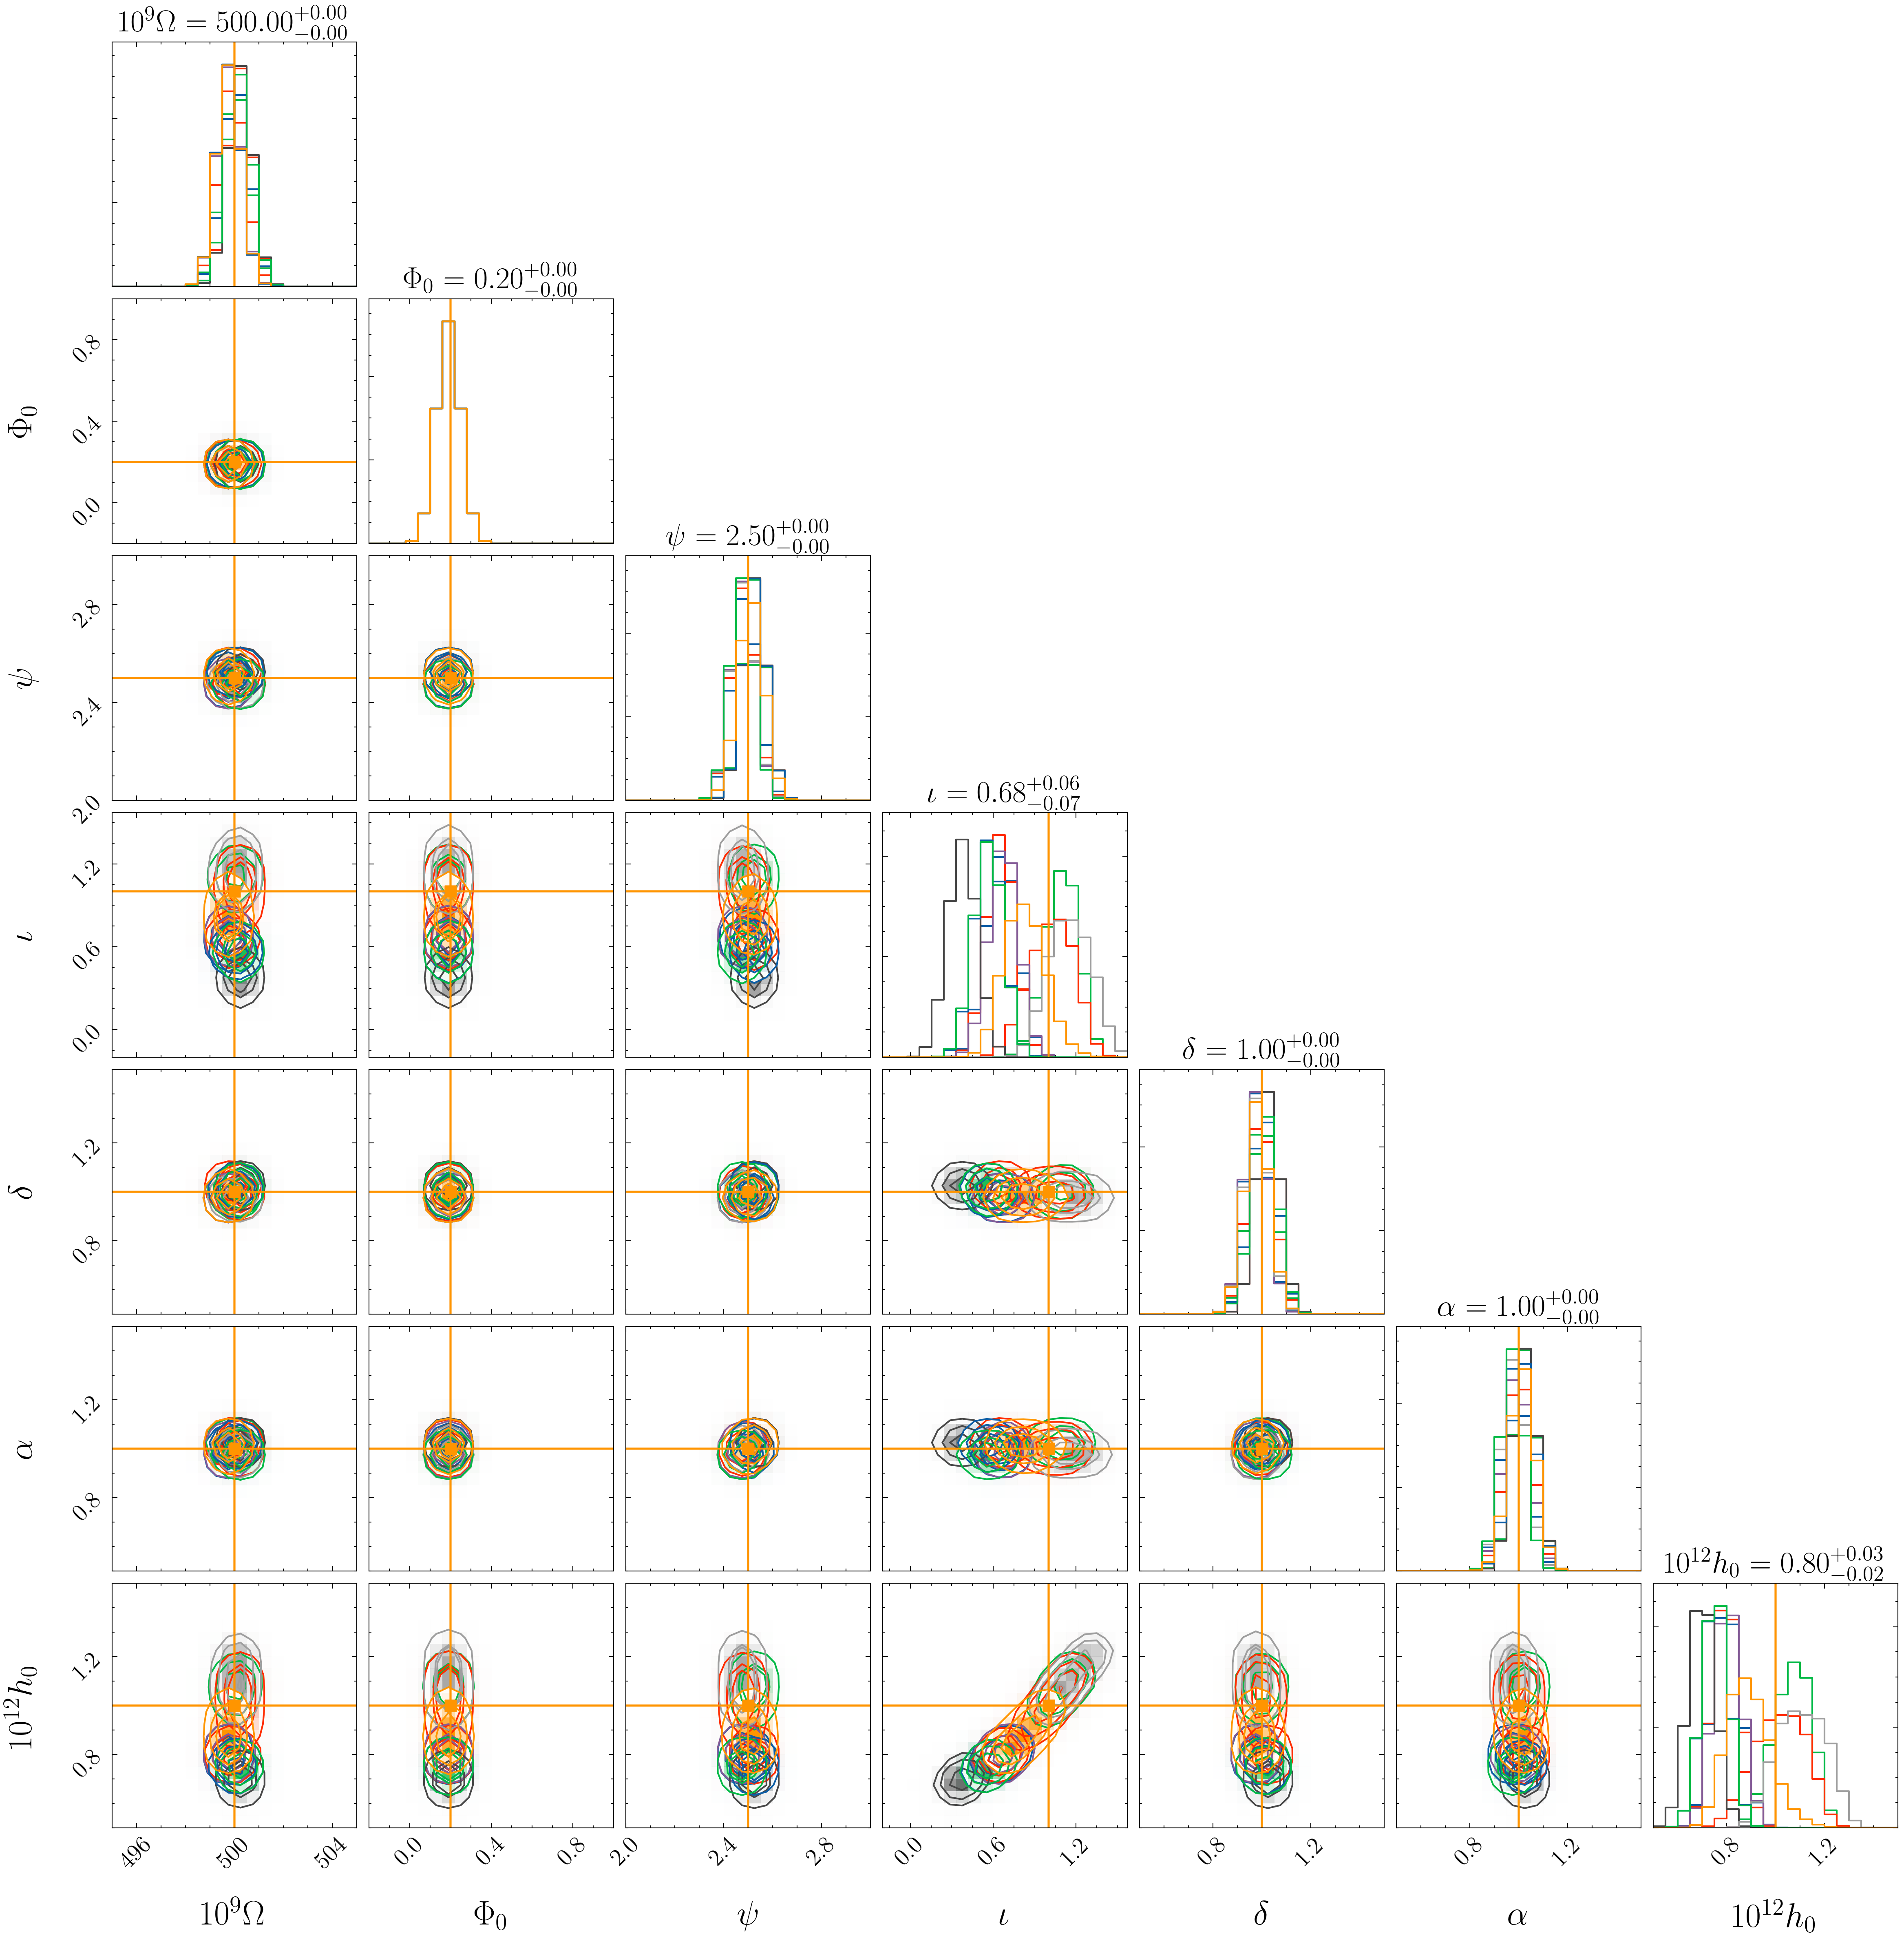
\includegraphics[width=\textwidth, height = \textwidth ]{images/corner_highSNR} 	
	\caption{}
	\label{fig:corner_high_snr_appendix}
\end{figure*}






	\begin{figure}
	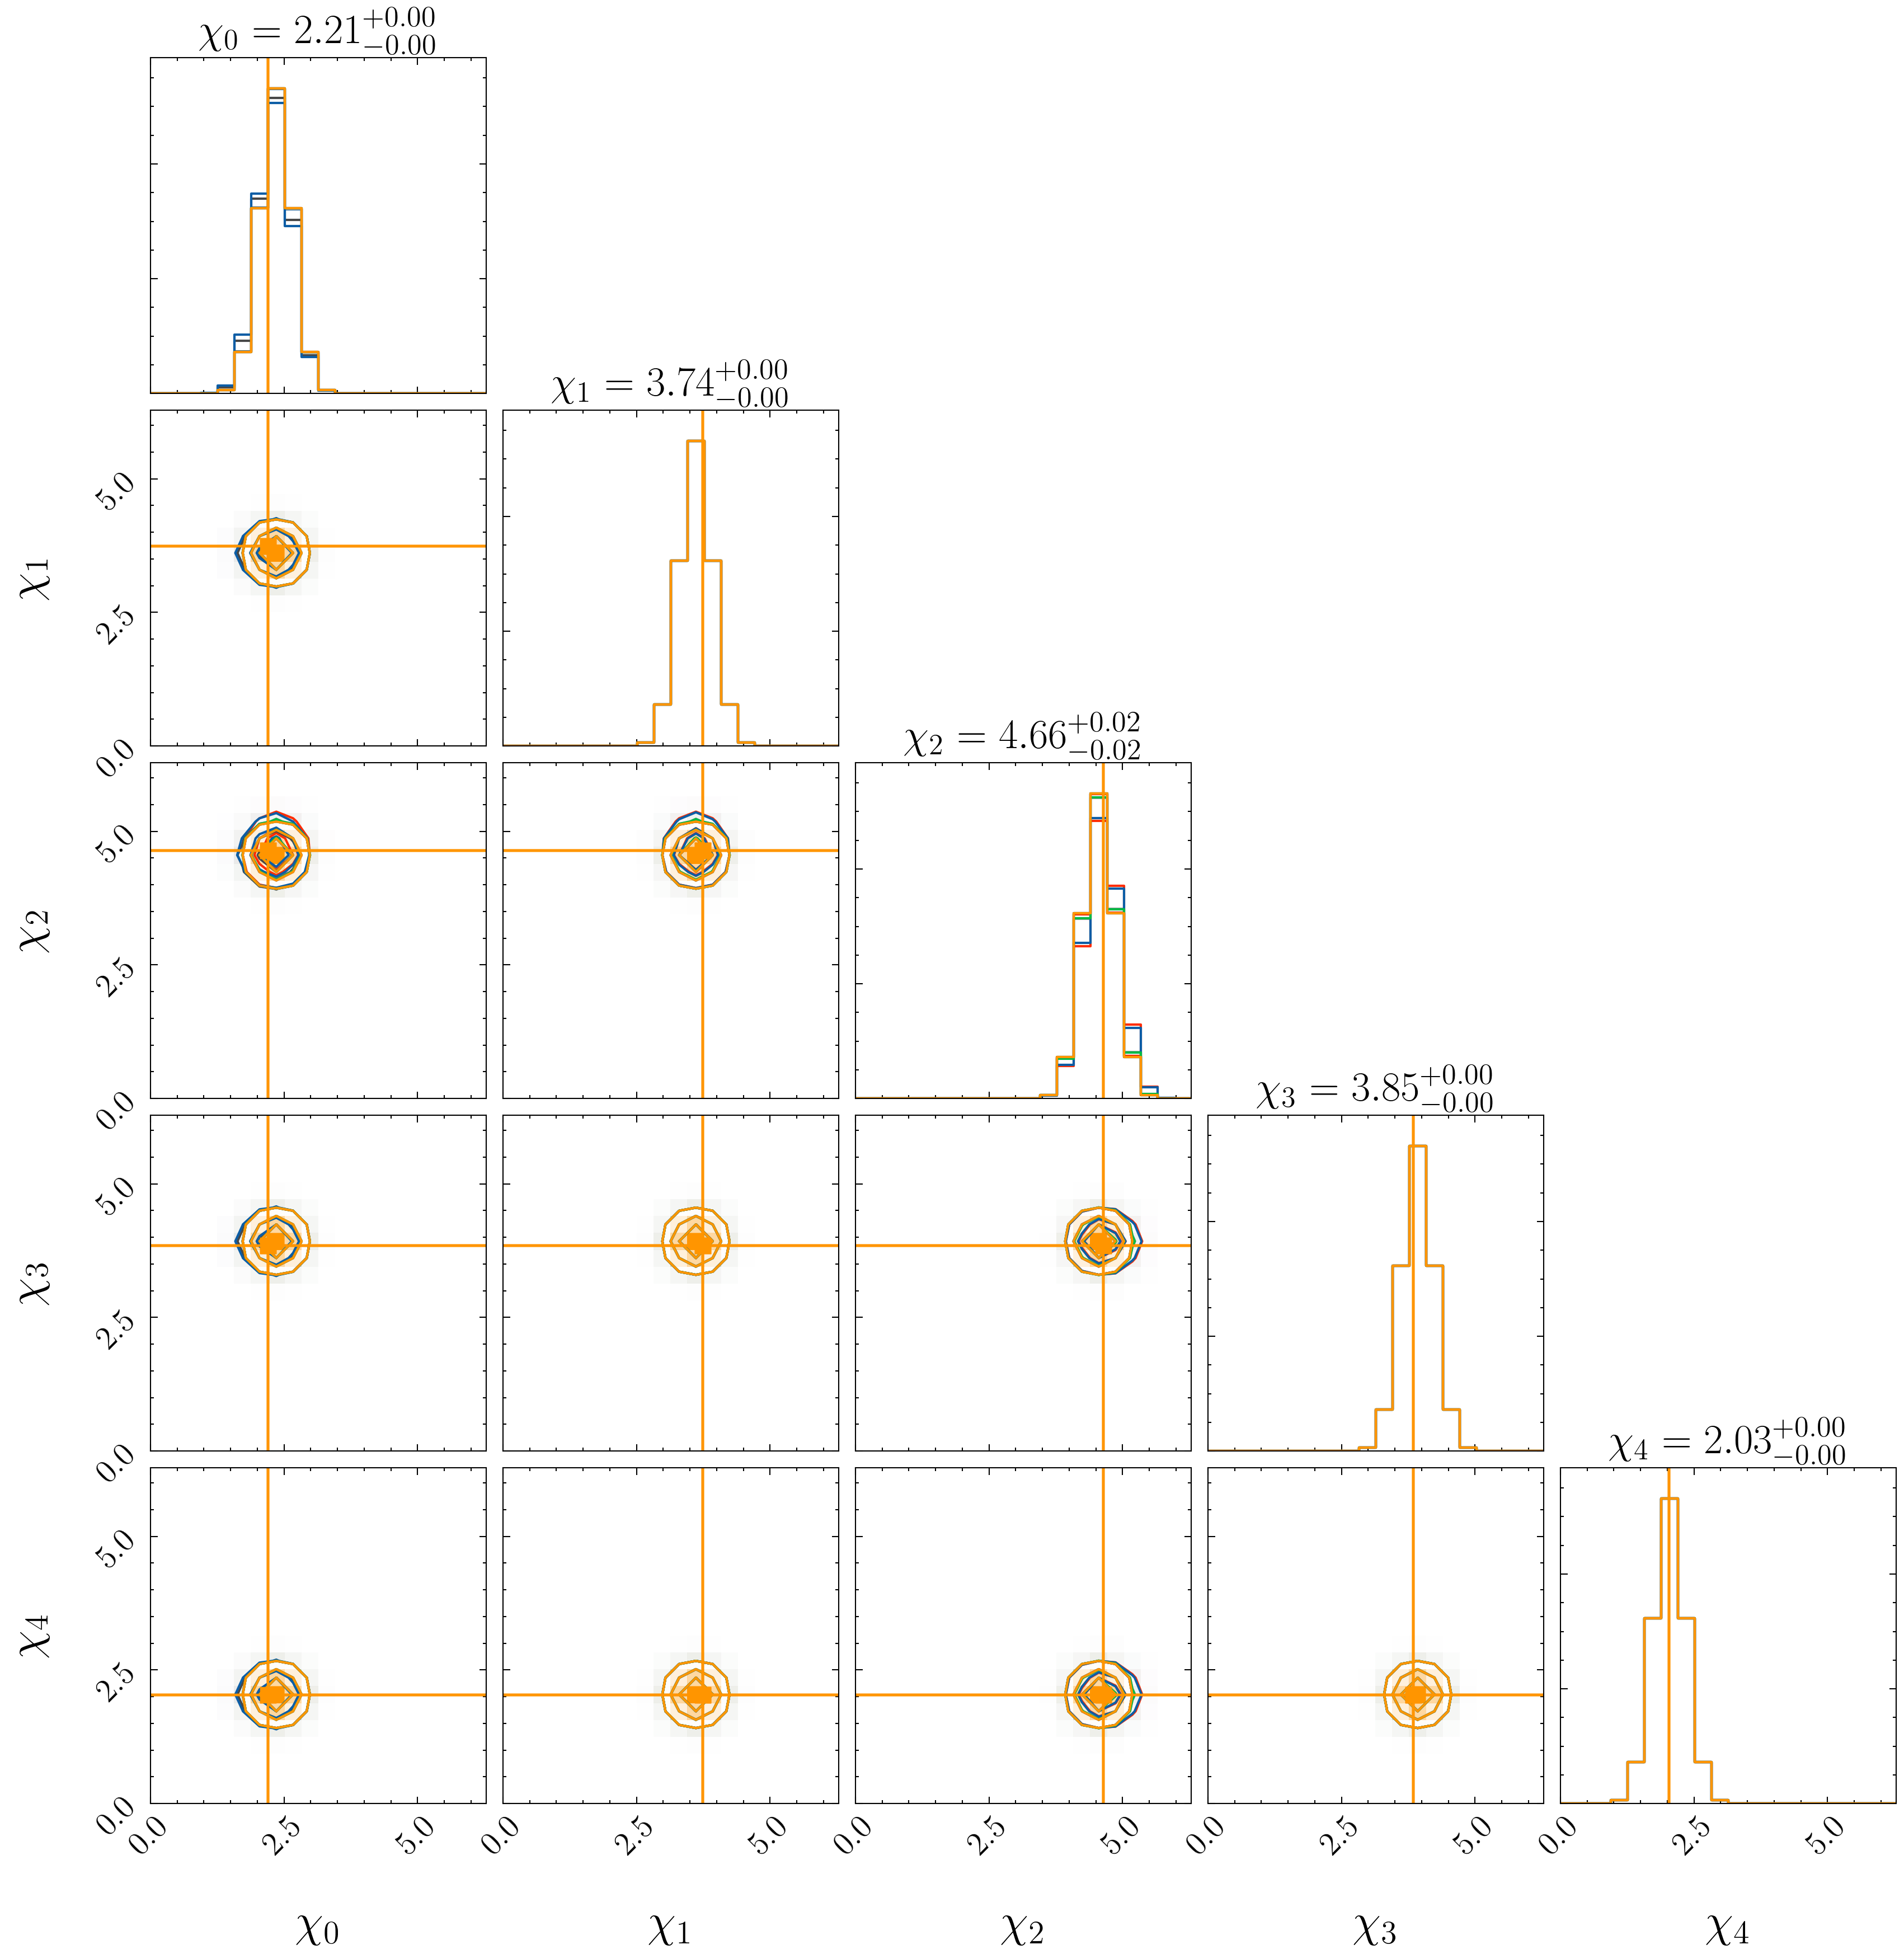
\includegraphics[width=\columnwidth, height = \columnwidth ]{images/corner_highSNR_chi} 	
	\caption{}
	\label{fig:corner_high_snr_appendix_chi}
\end{figure}



%
%\section{Multiple noise realisaitons and the Wasserstein distance}
%
%
%We can extend the analysis of these two points and consider 1000 noise realisations of $\boldsymbol{Y}$, beyond the \textcolor{red}{X} plotted in Figure \ref{fig:corner_plot_1}. As in Figure \ref{fig:corner_plot_1} we independently estimate the static parameters, $\boldsymbol{\theta}$ for each realisation and calculate $p({\boldsymbol{\theta'}} | {\boldsymbol{Y}})$. 
%
%
%
%
%To this end we start with the representative example in Table \ref{tab:parameters_and_priors} and generate $1000$ realisations of the process noise $\xi^{(n)}(t)$ and measurement noise $\varepsilon^{(n)}(t)$. For each realisation we 
%
%
%We now consider the complete set of $10^3$ noise realisations, going beyond the subset of nine realisations in the preceding discussion. We ask the question: how ``similar'' are the $10^3$ marginalized, one-dimensional posteriors computed for each of the seven parameters in ${\boldsymbol{\theta}}_{\rm gw}$? There is no unique way to answer this question. In this paper we appeal to the Wasserstein distance \citep[WD;][]{Wasserstein,Villani2009} from optimal transport theory, which defines an intuitive notion of similarity between probability distributions. The WD is a popular metric in machine learning \citep{2017arXiv170107875A}, climate modelling \citep{2022JCli...35.1215P,2023QJRMS.149..843K}, computational biology \citep{GONZALEZDELGADO2023168053} and geophysics \citep{2023GeoRL..5003880M}; a short review is presented in Appendix \ref{sec:wasserstein}. The WD measures the cost of an optimal strategy for moving probability mass between two distributions from position $x$ to position $y$, with respect to some cost function $c(x,y)$. In this paper we use the first WD moment, $W_1(\mu,\nu)$, which is defined and interpreted in Appendix \ref{sec:wasserstein}. Intuitively $W_1$ bounds the difference in the expectation value of a parameter selected from ${\boldsymbol{\theta}}_{\rm gw}$ with respect to the PDFs $\mu$ and $\nu$. Taking a concrete example, suppose that we infer two one-dimensional posterior distributions $\mu(\iota)$ and $\nu(\iota)$ for $\iota$, for two different realisations of the noise, and calculate $W_1(\mu, \nu) =0.5$ rad. Then we can infer $| \langle \iota \rangle_\mu - \langle \iota \rangle_\nu | \leq 0.5 \, {\rm rad}$. \newline 
%
%
%Table \ref{tab:Wasserstein} summarizes the WD between the $5\times 10^5$ pairs of one-dimensional posteriors across the $10^3$ realizations, for each of the seven parameters in ${\boldsymbol{\theta}}_{\rm gw}$. The median $W_1$ for each parameter is tabulated in the rightmost column and denoted by $W_{1,{\rm median}}$. As a percentage of the known, injected value, $W_{\rm 1,median}$ ranges from  0.2\% for $\Omega$ to 67\% for $\Phi_0$. These values quantify approximately the natural dispersion in parameter estimates when the analysis scheme is applied to real, astronomical data, where the true parameter values are unknown. Moreover, as a percentage of the prior domain, $W_{\rm 1,median}$ ranges from $8.1 \times 10^{-4}$ \% for $h_0$ to 2.7\% for $\psi$. These values confirm that the nested sampler converges reliably to a single, narrow peak without railing against the prior bounds for $10^3$ noise realizations. Further analysis of the WD is performed in Appendix \ref{sec:wasserstein}.
%
%\begin{table}
%	\centering
%	\begin{tabular}{ccll}
%		\toprule
%		Parameter & Injected value & Units & $W_{1, \rm median}$  \\
%		\hline
%		$\Omega$     &   $5 \times 10^{-7}$ & Hz & $10^{-9}$ \\
%		$\Phi_0$          & $0.20$ & rad & $0.13$ \\
%		$\psi$              & $2.50$ & rad & $0.16$ \\
%		$\iota$             & $1.0$ & rad & $0.14$ \\ 
%		$\delta$              & $1.0$  & rad & $0.09$ \\
%		$\alpha$          & $1.0$  & rad & $0.17$\\
%		$h_0$            & $5 \times 10^{-15}$ & --- & $8 \times 10^{-16}$ \\
%		\bottomrule
%	\end{tabular}
%	\caption{Median value of the Wasserstein distance $W_{1, \rm median}$, for each parameter in $\boldsymbol{\theta}_{\rm gw}$, calculated across the $10^3 \choose 2$ pairs of probability posteriors, for the $10^3$ noise realisations in Figure \ref{fig:pairwise_wasserstein}. $W_{1, \rm median}$ is generally smaller than the prior domain.}
%	\label{tab:Wasserstein}
%\end{table}
%
%



\section{Challenges of the pulsar term}\label{sec:psr_term_challenges}
In this section....

\begin{figure*}
	\includegraphics[width=\textwidth, height =0.5\textwidth ]{example-image-a}
	\caption{Logarithm of the one-dimensional likelihood $\mathcal{L}(\alpha)$ returned by the Kalman filter acting on synthetic data $\boldsymbol{Y}$. All other static parameters of $\boldsymbol{\theta}$ are held constant at their true injected values. In the left-hand panel the Kalman filter uses Equation \eqref{eq:g_func_trig} to calculate $\mathcal{L}(\alpha)$, i.e. inclusive of the pulsar terms. In the right-hand panel the Kalman filter uses Equation \ref{eq:g_func_trig_earth}, i.e. just the Earth terms. The vertical dashed lines indicate the true injected value of $\alpha$ ($=1.0$ rad) used to generate $\boldsymbol{Y}$. The inset plot covers the region $1.0 - 10^{-4} \le \alpha \le 1.0 +10^{-4}$ rad. In the left hand panel $\mathcal{L}(\alpha)$ is very noisy, though a smooth concave optima exists on scales $\mathcal{O}(10^{-4})$ rad. This noise hampers the ability of sampling algorithms to converge to a posterior distribution. Conversely, in the right hand panel $\mathcal{L}(\alpha)$ is globally smooth. }
	\label{fig:likelihood_comparison}
\end{figure*}




To elucidate the complications introduced by including the pulsar term, we generate some noisy synthetic data $\boldsymbol{Y}$ using the methods outlined in K23. $\boldsymbol{\theta}_{\rm gw}$ are chosen arbitrarily, with $\alpha = 1.0 $ rad.
The choice of $\boldsymbol{\theta}_{\rm psr}$ corresponds to the 47 pulsars in the 12.5 year NANOGrav data set  \citep{2020ApJ...905L..34A}. We run the Kalman filter using the measurement equation inclusive of the pulsar terms, Equation \eqref{eq:g_func_trig} on $\boldsymbol{Y}$ for different values of $\alpha$, $ 0.0 \le \alpha \le \pi$ rad. We obtain a curve $\mathcal{L}(\alpha)$, which is plotted in the left hand panel of Figure \ref{fig:likelihood_comparison} (blue curve). The dashed grey line indicates the injected value of $\alpha$ (= 1.0 rad). The inset plot shows a zoomed-in section of $\mathcal{L}(\alpha)$ within the region $ 1.0 - 10^{-4} \le \alpha \le 1.0 +10^{-4}$ rad. \newline 

There are two important features to discuss in the left-hand panel of Figure \ref{fig:likelihood_comparison}. The first is that on scales of order the width of the prior $\pi(\alpha)$ (i.e radians), the curve of $\mathcal{L}(\alpha)$ is very noisy. Similar noisy curves are obtained for $\mathcal{L}(\Omega)$ and $\mathcal{L}(\delta)$. For all other static parameters, the $\mathcal{L}(\Theta)$ curves are smooth and globally concave. The second is that despite being noisy, a true likelihood maximum coincident with the injected value does exist and is locally concave on scales $\mathcal{O} \left( 10^{-4}\right)$ radians. This means that whilst it is theoretically possible to use likelihood-based methods for Bayesian estimation of $\alpha$, in practice the computation is intractable since the noise in the likelihood curve inhibits sampling algorithms to reliably converge to a definitive posterior. Moreover, $\mathcal{L}(\alpha)$ is only a one-dimensional function. The challenge for sampling algorithms is further exacerbated when we consider the three-dimensional parameter space in $\alpha - \delta - \Omega$, or the full $7 + 5N$ dimensions of Section \ref{sec:ss_params}. \newline 

Why do $\alpha$, $\delta$ and $\Omega$ exhibit noisy $\mathcal{L}(\Theta)$ curves whereas other static parameters do not? These parameters appear in the pulsar term as a product in the pulsar-dependent phase correction $\Omega \left(1 + \boldsymbol{n}\cdot \boldsymbol{q}^{(n)} \right)  d^{(n)}$, where we remind the reader that $\boldsymbol{n} = \boldsymbol{n}(\delta, \alpha)$. Over the typical pulsar distances $d^{(n)} \sim 1$ kpc, a 10 nHz GW can accumulate $10^3$ cycles. This creates a confusion problem when taking the cosine of  $\Omega \left(1 + \boldsymbol{n}\cdot \boldsymbol{q}^{(n)} \right)  d^{(n)}$ since we do not know how many cycles the wave has gone through, modulo $2 \pi$. \textcolor{red}{TK: this explanation is rubbish! How can we say this better?}. Conversely, if we drop the pulsar term,  the $\mathcal{L}(\alpha)$ curve (as well as $\mathcal{L}(\Omega)$ , $\mathcal{L}(\delta)$   )
This is shown by the orange curve in the right-hand panel of Figure \ref{fig:likelihood_comparison} where we plot $\mathcal{L}(\alpha)$, analogous to the left-hand panel, but now use Equation \ref{eq:g_func_trig_earth} in our Kalman filter (i.e. just the Earth terms) rather than the full Equation \ref{eq:g_func_trig}. In this case there is no confusion regarding the number of cycles the wave has gone through over a distance $d^{(n)}$ and the curve is smooth.




In this section we present a new method to infer $\boldsymbol{\theta}$ and calculate the marginal likelihood (i.e. the model evidence). In Section \ref{sec:kalman_filter} we outline how noisy measurements of the pulsar frequency, $f_{\rm m}^{(n)}(t)$, can be used to estimate the hidden state sequence, $f_{\rm p}^{(n)}(t)$, using a Kalman filter. In Section \ref{sec:nested_sampling} we demonstrate how to deploy the Kalman filter in conjunction with a nested sampling technique to perform Bayesian inference. Model selection and the specification of the null model are described in Section \ref{sec:model_selection}. A complete summary of the workflow is presented in Section \ref{sec:methodsummary}. The method complements traditional PTA analyses because (i) it does not assume a specific functional form (e.g.\ power law) for the power spectral density of the TOA fluctuations; and (ii) it infers ${\boldsymbol{\theta}}$ conditional on the specific, time-ordered, random realization of the noise corresponding to the observed sequence of TOAs rather than on ensemble-averaged quantities like the power spectral density.








%See https://arxiv.org/pdf/2102.12478.pdf for a good NS explanation







%
%\section{Model selection}\label{sec:model_selection}
%The evidence integral $\mathcal{Z}$ returned by nested sampling is the probability of the data $\boldsymbol{Y}$ given a model $\mathcal{M}_i$. We compare competing models via a Bayes factor,
%\begin{equation}
%	\beta = \frac{\mathcal{Z}(\boldsymbol{Y} | \mathcal{M}_1)}{\mathcal{Z}(\boldsymbol{Y} | \mathcal{M}_0)} \ . \label{eq:bayes}
%\end{equation}
%Throughout this work we take $\mathcal{M}_1$ to be the state-space model that includes the presence of a GW. $\mathcal{M}_0$ is the null model, which assumes no GW exists in the data, and is equivalent to setting $g^{(n)}(t)=1$ in Equations \eqref{eq:g_func} and \eqref{eq:g_func_trig}. The Bayes factors we quote in this work therefore quantify whether the data supports evidence for a GW signal compared to there being no GW signal present.
%
%







%%%%%%%%%%%%%%%%%%%%%%%%%%%%%%%%%%%%%%%%%%%%%%%%%%


% Don't change these lines
\bsp	% typesetting comment
\label{lastpage}
\end{document}

% End of mnras_guide.tex
